\documentclass[12pt]{report}

\title{Topic modeling on EU and the USA research projects}
\author{Maria Iliadi}

\renewcommand{\thesection}{\arabic{section}}

\setcounter{secnumdepth}{4}
\setcounter{tocdepth}{4}
\setlength{\parskip}{1em}

\usepackage[justification=centering]{caption}
\usepackage{amsfonts}
\usepackage{graphicx}
\usepackage{cite}
\usepackage{algorithm2e}
\usepackage{url}
\usepackage{subfig}
\usepackage{listings}
\usepackage[utf8]{inputenc}
\usepackage{color}
\usepackage{geometry} 
 
\definecolor{codegreen}{rgb}{0,0.6,0}
\definecolor{codegray}{rgb}{0.5,0.5,0.5}
\definecolor{codepurple}{rgb}{0.58,0,0.82}
\definecolor{backcolour}{rgb}{0.95,0.95,0.92}
 
\lstdefinestyle{mystyle}{
    backgroundcolor=\color{backcolour},   
    commentstyle=\color{codegreen},
    keywordstyle=\color{magenta},
    numberstyle=\tiny\color{codegray},
    stringstyle=\color{codepurple},
    basicstyle=\footnotesize,
    breakatwhitespace=false,         
    breaklines=true,                 
    captionpos=b,                    
    keepspaces=true,                 
    numbers=left,                    
    numbersep=5pt,                  
    showspaces=false,                
    showstringspaces=false,
    showtabs=false,                  
    tabsize=2
}
 
\lstset{style=mystyle}

\begin{document}

\begin{titlepage}
	\centering
	
\includegraphics[width=0.8\textwidth]{figs/logo.jpg}\par\vspace{4cm}
	{\scshape\Large MSc thesis\par}
	\vspace{1.5cm}
	{\Large\bfseries Topic modeling on EU and the USA research projects\par}
	\vspace{2cm}
	{\Large Maria Iliadi\par}
	\vfill
	supervised by\par
	Assoc.Prof.~Panos Louridas

	\vfill

% Bottom of the page
	{\large \today\par}
\end{titlepage}
\tableofcontents

\begin{abstract}
The purpose of this work is to better identify, quantify and understand themes
in research and innovation over the last 22 years, and to provide valuable
knowledge about the research trends nowadays. A way to approach the issue is
through the projects supported by funding agencies. In particular, public data
are available for the projects funded under the European Union Framework
Programmes, and for project funded by the NSF in the United States. The data
include project descriptions, so it is possible to investigate, based on these
textual data, the research topics that were actually funded over the last two
decades. We first introduce the concept of Latent Dirichlet allocation and its
application in topic modeling in projects funded in the two regions from 1994
to 2017. We will then proceed to show the differences between the two regions in
terms of topic similarity and topic evolution over time. We will discuss both
policy implications, what has been funded over the years, as well as technical
ones, how can one handle such datasets and extract information from them.
\end{abstract}


\section{Introduction}
Research is the foundation on which knowledge and new technologies emerge and
support our welfare. Scientific research brings together observation, knowledge
and data to solve problems, invent solutions and develop new products. In our
globalized world, the shared commitment for excellence in science has a major
impact to our well being and it's important to support research and development.
Over the last years, many projects from different domains are getting funded for
research and innovation.

Nowadays, there are many funding opportunities for researchers. For instance,
European Union countries are encouraged to invest 3\% of their GDP in research
and development by 2020. EU's latest research programme, Horizon 2020, allows
researchers to identify new opportunities and directions in almost any field of
research. The programme's goals are to strengthen the EU's position in science,
support industrial innovation and address social concerns, such as climate
change, green transportation and energy.

Another funding agency that actively promotes the progress of science is the
National Science Foundation in the United States of America. NSF supports
research in all the non medical fields of science \& engineering and aims to
advance the national health and prosperity. It finds approximately 24\% of the
federally supported research conducted by the USA's colleges and universities.

With our work, we aim to investigate the evolution of scientific research in the
EU and the US. In other words, we attempt to identify which subjects are more
likely to get a funding, based on the previous focus the two regions in research
fields. In order to answer these questions, we tried to gain some insights from
the projects that got funded the last two decades under the EU Framework
Programmes and the NSF in USA.

When researchers apply for a funding, one of the first steps they do is to
identify an interesting subject of the many possible topics of scientific
investigation. The topic(s) of a project is always described in the project's
abstract/description. Obtaining these abstracts, one can possibly investigate
the topics of the projects and find the subjects that are being addressed and
gain some information regarding the popularity of the topics among others.

In this work, we discover topics and their evolution from 1994 to 2017, using
the projects' abstracts that got funded this period. Using a topic model, we
extract a set of topics and investigate the changes in the content per
year/framework programme. These topics are used to gain insight into some of the
research that occurs the last two decades. Our goal is to share these insights
with researchers and encourage them to develop better strategies to establish
themselves as more effective researchers globally, by choosing a subject that is
more likely to get a funding.

In section 2, we briefly talk about the papers that mostly influenced our study.
Section 3 introduces some basic concepts in topic modeling and we describe the
model that we used for topic extraction, Latent Dirichlet Allocation, which is a
statistical generative model for documents. In section 4 we provide information
about the dataset structure and the methodology that we followed in our
analysis. In section 5 we interpret the results of our analysis, discuss the
evolution of the topics over time and the differences between the two regions'
topics based on their similarity. Finally, section 6 summarizes our work and
section 7 suggests some future work.

\section{Related work}

This chapter surveys previous work in topic modeling on scientific data. Topic
modeling algorithms provides a suite of algorithms to discover hidden thematic
structure in large collections of texts and can be adapted to many kinds of
data. These algorithms can be used to summarize, visualize and explore a
collection of documents. The papers listed below are applying a Latent Dirichlet
Allocation model in an interesting approach on their corpus.

D.Blei's research focuses on probabilistic topic models, Bayesian methods and
approximate posterior inference. In his work "Introduction to Probabilistic
Topic Models",\cite{Blei11introductionto} he describes the basic ideas behind
LDA and applies the model to articles from the journal "Science". The model
assumes that the topics are generated first, before the documents and that the
documents exhibit multiple topics, but each one of them exhibit those topics in
different proportion. In our implementation we also use the LDA model and we
follow a similar approach, since we don't use any previous information about the
subjects that run through our dataset and the documents are not labeled with
keywords or topics. The topic distributions arise by computing the hidden
structure that resembles the thematic structure of the collection.

The paper that mostly influenced our work is "Finding Scientific Topics", by
T.Griffiths and M.Steyvers.\cite{griffiths_steyvers04} They investigated
abstract data from articles published in the Proceedings of the National Academy
of Sciences (PNAS) from 1991 to 2001 and compared research topics obtained from
topic modeling with existing categories. In our implementation, we also use 
the abstracts of the projects as documents for the model.

Griffiths and Steyvers describe LDA and present a Markov Chain Monte Carlo
algorithm for inference in the model, illustrating the operation of the
suggested algorithm on a small dataset, and then on a larger corpus of PNAS
abstracts. Finally, they define the dynamics of the topics as a means of gaining
insight into the dynamics of science. As "hot" topics are identified the topics
that appear more frequently over the years (positive linear trend), and as
"cold" the ones that appear less frequently (negative linear trends over time).
We also analyze the topics over time, in order to highlight potential trends in
scientific research in EU and USA.

Inspired by Griffiths and Steyvers, L.Sun and Y.Yin wrote a paper, "Discovering
themes and trends in transportation research using topic modeling",
\cite{Sun201749} about topic modeling in transportation research. 
Considering approximately 17000 abstracts of articles published on 22 
leading journals in transportation research as documents, they infer 50 
topics by using LDA. Compared to "Finding scientific topics", Sun and 
Yin use more than one journal (22 popular journals) and they
investigate the journal-topic distribution and journal similarity. In our
analysis, we identify the EU and the USA as 2 regions (like 2 different journals),
with different proportions of documents-projects, and we visualize the topic
similarity of the two regions per framework programme.

To best of our knowledge, there is no work done in the field of topic modeling
on scientific projects between EU and USA. There is limited information from
European Commission about the evolution and the results of the projects provided
by the official website.


\section{Theoretic background}

In this chapter we will present some basic theoretic background about topic
modeling. To deal with extensive text body, machine learning researchers have
developed topic modeling: a suite of methods that analyze the words of the
original text to discover the themes that run through the data and detect
hidden semantic structures by analyzing a corpus. By marking up the documents
using these topics and by using the resulting structure, the model can be used
for organization, finding similar documents, or any other similar tasks. A
topic is here defined as a probability distribution of words, meaning that
certain words are more likely within a certain topic. Since the topics emerge
from the analysis of the original texts, topic modeling algorithms do not
require any prior annotations or labeling of the documents.\cite{Blei11introductionto}

In order to apply a topic model to our data, the first question we must answer
is how to represent documents. For understanding of natural language one must
obviously preserve the order of the words in documents. However, for many
large-scale data mining tasks, it is sufficient to use a simple representation
that loses all information about word order. Given a collection of documents,
the first task to perform is to identify the set of all words used at least
once in at least one document. This set is called the vocabulary. Often, we
reduce the size of the vocabulary by keeping only words that are used in at
least a small percentage of the documents. Words that are found only once are
often misspellings or other mistakes. Although the vocabulary is a set, we fix
an arbitrary ordering for it so we can refer to word 1 through word $m$ where
$m$ is the size of the vocabulary. Once the vocabulary has been fixed, each
document is represented as a vector with integer entries of length $m$. If this
vector is $x$ then its $j$-th component $x_j$ is the number of appearances of
word $j$ in the document. The length of the document is $n=\sum\limits_{j=1}^m
x^j$.

Many applications of topic modeling also eliminate from the vocabulary so
called “stop” words. These are words that are common in most documents and do
not correspond to any particular subject matter. They include pronouns (you,
he, it), connectives (and, because, however), prepositions (to, of, before),
and auxiliaries (have, been, can, should). Stop words may also include generic
nouns (amount, part, nothing) and verbs (do, have). A collection of documents
is represented as a two-dimensional matrix where each row describes a document
and each column corresponds to a word. Each entry in this matrix is an integer
count; most entries are zero. It makes sense to view each column as a feature.

Some further common concepts and terms in topic modeling: 
\begin{itemize}
\item[] A \textit{word} is defined as an item from a vocabulary indexed from 
${1, ..., V}$, where V is the size of the vocabulary. All words are 
represented as unit-basis vectors with one component equal to one and 
the rest equal to zero.
\item[] A \textit{document} is a collection of words denoted by $w = {w_1, ..., w_N}$, 
where $w_n$ is the $n$th word and $N$ is the total number of words in the 
collection.
\item[] A \textit{corpus} is a collection of documents in a dataset. It is denoted 
$D = {w_1,..., w_M}$, where $w_m$ is the $m$th document in the corpus and 
$M$ is the total number of documents.
\item[] \textit{Latent variables} are variables that may not be directly observed, 
unlike observable variables. Latent variables can instead be inferred 
from other observable variables.
\item[] \textit{Polysemy} is the capacity for a word to have multiple related meanings. 
An example of this is the word “plant” which can mean a living organism of 
the kind exemplified by trees, herbs etc., or a place where an industrial or
manufacturing process takes place.
\item[] \textit{Synonymy} is the capacity for several words to have similar meanings such as
the words “buy” and “purchase”.
\end{itemize}

\subsection{Some probability concepts}

\subparagraph{Prior and posterior distributions}

When introducing the Latent Dirichlet Allocation in section 2.2.3, we 
will be using the terms prior and posterior probabilities and 
likelihood function:

\begin{itemize}
\item The prior probability distribution of and uncertain quantity is the 
probability distribution that express the value of this quantity before 
some evidence is taken into account.
\item The posterior probability is the conditional probability after some 
evidence is taken into account.
\item The likelihood function of a set of parameters given some outcome 
is equal to the probability of observing said outcome given those 
parameter values.
\end{itemize}

If the prior and the posterior distributions are in the same distribution
family, then the prior and posterior are called conjugate distributions and the
prior is called a conjugate prior for the likelihood function.

Given a prior $p(\theta)$ and observations x with the likelihood 
$p(x \mid \theta)$, the posterior is defined as:

\begin{equation}
p(\theta \mid x) = \frac{p(x \mid \theta) p(\theta)}{p(x)}
\end{equation}


\subparagraph{Jensen Inequality}

In the context of probabilities, the Jensen Inequality is stated as follows: 
If X is a random variable and f a convex function then:

\begin{equation}
f(\mathbb{E}[X]) \leq \mathbb{E}[f(X)]
\end{equation}

And, if f is a concave function the inequality turns:

\begin{equation}
f(\mathbb{E}[X]) \geq \mathbb{E}[f(X)]
\end{equation}


\subparagraph{Kullback-Leibler (KL) divergence}

When formulating the optimization problem in Latent Dirichlet Allocation we 
will use the KL divergence to express the optimization problem. The KL divergence 
is a measure of the difference between two probability distributions $P$ and $Q$. 
It is important to note
that the KL divergence is not symmetrical in $P$ and $Q$ so it's not a metric.

The KL divergence can be interpreted as a way to express the amount of 
information lost when $Q$ is used to approximate $P$.

Given two continuous distributions $P$ and $Q$ the KL divergence is defined as follows:

\begin{equation}
D_{KL}(P \mid \mid Q) = \int_{-\infty}^{+\infty} p(x) log\frac{p(x)}{q(x)}dx
\end{equation}

This can also be expressed using the definition of expectation (and expressing the 
log of a division as difference of log) as:

\begin{equation}
D_{KL}(P \mid \mid Q) = \mathbb{E}_{p}[log p(x)] - \mathbb{E}_{p}[log q(x)]
\end{equation}

This is the expression we will use later on instead of the definition. We present 
now the two probability distributions we will be using when we define the different 
models in this work: the \textbf{Multinomial} and the \textbf{Dirichlet} distributions. 


\subparagraph{Multinomial Distribution}

Once we have a representation for individual documents, the natural next step
is to select a model for a set of documents. Given a training set of
documents, we will choose values for the parameters of a probabilistic model
that make the training documents have high probability. Then, given a test
document, we can evaluate its probability according to the model. The higher
this probability is, the more similar the test document is to the training set.


The probability distribution that we use is the multinomial. In probability 
theory, the multinomial distribution is a generalization of the binomial 
distribution. For example, it models the probability of counts for rolling 
a k-sided dice n times. For n independent trials each of which leads to a 
success for exactly one of k categories, with each category having a given 
fixed success probability, the multinomial distribution gives the 
probability of any particular combination of numbers of successes for the 
various categories\footnote{\url{https://en.wikipedia.org/wiki/Multinomial_distribution}}. 

Mathematically, this distribution is: 

\begin{equation}
p(x;\theta) = \left(\frac{n!}{\prod\limits_{j=1}^m x^j!}\right)\left
(\prod\limits_{j=1}^m \theta_j^{x_j}\right)
\end{equation}

where the data $x$ are a vector of non-negative integers and the parameters
$\theta$ are a real-valued vector. Both vectors have the same length $m$.
Intuitively, $\theta_j$ is the probability of word $j$ while $x_j$ is the count
of word $j$. Each time word $j$ appears in the document it contributes an amount
$\theta_j$ to the total probability, hence the term $\theta_j^{x_j}$. The
components of $\theta$ are non-negative and have unit $\sum\limits_{j=1}^m
\theta_j = 1$.

Like any discrete distribution, a multinomial has to sum to one, where the sum
is over all possible data points. Here, a data point is a document containing
$n$ words.\cite{Huang_maximumlikelihood}


\subparagraph{Dirichlet distribution}

The Dirichlet distribution is a way to model random probability mass functions
(PMFs)\footnote{If you roll 1000 dice, the theoretical odds of any particular
number showing up (i.e. a 1, 2, 3, 4, 5, or 6) are 1/6. However, you won't get
that exact distribution in a real experiment due to manufacturing defects. If
you have ten dice, each die will have its own probability mass function (PMF).}
for finite sets. It is also sometimes used as a prior in Bayesian statistics.
The Dirichlet is the multivariate generalization of the beta distribution. It
is an extension of the beta distribution for modeling probabilities for two or
more events; when the result of the event has only 2 values, the Dirichlet
distribution is equal to the beta distribution.

The Dirichlet distribution is a prior for the multinomial distribution. This
means that if the prior distribution of the multinomial parameters is Dirichlet
then the posterior distribution is also a Dirichlet distribution (with
parameters different from those of the prior).

The Dirichlet process is a way to model randomness of a probability mass
function (PMF) with unlimited options (e.g. an unlimited amount of dice in a
bag). The process is similar Polya's Urn\footnote{\url{http://www.statisticshowto.com/dirichlet-distribution/}}, only instead of having a set number
of ball colors you have an unlimited amount:

\begin{itemize}
\item Start out with an empty urn.
\item Randomly pick a colored ball and place it in the urn.
\item Then choose one option:
\begin{enumerate}
\item Randomly pick a colored ball and place it in the urn.
\item Randomly remove a colored ball from the urn, then put it back with another 
ball of the same color.
\end{enumerate}
\end{itemize}
 
As the number of balls in the urn increase, the probability of picking a new
color decreases. The proportion of balls in the urn after an infinite amount of
draws is a Dirichlet process.


\subsection{Basic models in topic modeling}

First, we'll introduce some basic models for topic modeling. The Latent Semantic
Indexing, or LSI, was presented by Deerwester et al. in 1990. The model manages
to deal with the problem that multiple terms can refer to the same meaning,
i.e. synonymy. However, it is not as successful regarding polysemy. The reason
is that every term is represented as just one point in the so-called latent
semantic space. Furthermore, a word that can mean two or more different things
is represented as a weighted average of the different meanings.
 
After LSI was introduced, Hofmann presented the Probabilistic Latent Semantic
Indexing, or PLSI model. PLSI is a topic model where each word in a
document is generated from a single topic which results in that each document
in a corpus can be represented with a topic distribution. Later, in 2003 Blei et
al. presented the Latent Dirichlet Allocation, or LDA. As opposed to PLSI, LDA
is a statistically generative model for documents where each word in a document
can be generated by all topics.

\subsubsection{Latent Semantic Indexing (LSI)}

Latent Semantic Indexing was one of the earliest methods for finding
relationships between documents and the words that occur in them.\cite{Deerwester90indexingby} In LSI a
term-document matrix is created by analyzing the corpus, where the rows
correspond to words and columns to documents. Each element in this sparse
matrix describes the number of times a word occurs in a document but this term
count can also be weighted with for instance TF-IDF. Letting each word
represent a dimension in a very high dimensional space, a document can be seen
as a vector with components corresponding to its weighted term counts.
\cite{Salton:1988:TAA:54259.54260}

A low-rank approximation of the term-document matrix is created using Single
Value Decomposition, SVD, which creates new dimensions, called concepts, as
linear combinations of the original words. This allows similarity measures and
clustering methods by reducing the volume of the word space and thus making
this space more densely populated.

The drawbacks with LSI are mainly the lack of a statistical foundation in the
model. LSI is based on linear algebra instead of probabilistic modeling leaving
it with a small toolbox for what can be achieved using the model.
	

\subsubsection{Probabilistic Latent Semantic Indexing (PLSI)}


Probabilistic Latent Semantic Indexing evolved from LSI and uses the same
concept of finding a lower rank approximation of the term-document occurrence
matrix. The difference is that instead of being based on linear algebra, PLSI
is based on a mixture decomposition using a latent class model.
~\cite{Hofmann:1999:PLS:312624.312649} PLSI associates an unobserved class 
variable $z$ with each document-word observation pair (\textbf{w},$
w)$. This $z$ can be seen as a topic, since it is a probability distribution
over words. As a generative model, PLSI can be defined in the following way 
for a corpus $D$:

\begin{enumerate}
\item Pick a document \textbf{w} with probability $p($\textbf{w}$)$
\item For each of the $N$ words in \textbf{w}:
\begin{description}
\item (a) Pick a topic $z$ with probability $p(z|$\textbf{w}$)$
\end{description}
\begin{description}
\item (b) Generate a word $w$ with probability $p(w|z)$
\end{description}
\end{enumerate}
\begin{center}
\begin{figure}[h]
\centering
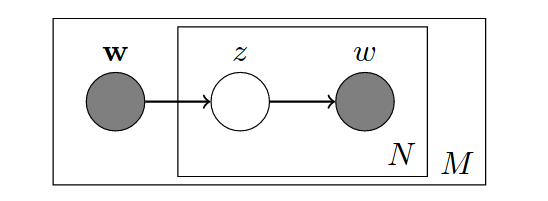
\includegraphics[width=0.6\textwidth]{figs/PLSI_plate_notation.png}
\caption{Plate notation representing the PLSI model. \textbf{w} is the document 
index, $z$ is the topic drawn for the word $w$ from the topic distribution of 
the document}
\end{figure}
\end{center}
The result from PLSI is that every document is represented as mixing proportions
for the topics, given by $p(z|$\textbf{w}$)$. Even though PLSI is generative for 
the analyzed corpus, it is not generative for new documents, which means is that
there is no clear way of assigning probability to a document that is not part
of the training data.\cite{blei2003latent} Another problem is that the number 
of parameters in the model grows linearly with the number of documents.


\subsubsection{Latent Dirichlet Allocation (LDA)}

LDA is a topic model that was first presented as a graphical model for topic
discovery by David Blei, Andrew Ng, and Michael I. Jordan in 2003. The basic
idea is that documents exhibit multiple topics. LDA is a generative statistical
model that allows sets of observations to be explained by unobserved groups
that explain why some parts of the data are similar. For example, if
observations are words collected into documents, it posits that each document
is a mixture of a small number of topics and that each word's occurrence is
attributable to one of the document's topics.\cite{Blei11introductionto}

This is similar to PLSI, except
that in LDA the topic distribution is assumed to have a Dirichlet prior. 
In practice, this results in more reasonable mixtures of topics in a
document. The reduced document description result in PLSI is a vector where
each element describes the mixing proportion for a topic. A limitation with
PLSI is that there is no generative model for these proportions, making it
difficult to handle unseen documents. The Latent Dirichlet Allocation model
tries to solve this limitation by setting a Dirichlet prior on the topic
distribution.\cite{blei2003latent}
 
Suppose that we have a collection of documents, and we want to find an
organization for these, i.e. we want to do unsupervised learning. A common way
to do unsupervised learning is to assume that the data were generated by some
probabilistic process, and then to infer the parameters of this process. The
generative process is a specification of a parametrized family of
distributions. Learning is based on the principle of maximum likelihood, or
some refinement of this principle such as maximum a posterior probability.
 
The basic idea in LDA is that we define a topic to be a Dirichlet distribution
over a fixed vocabulary. Technically, the model assumes that the topics are
generated first, before the documents.\cite{Blei11introductionto} Now for 
each document in the collection, we generate the words in a two-stage process:

\begin{algorithm}[H]
\SetAlgoNoLine
1. Randomly choose a distribution over topics.

2. 
\For{each word in the document}{
	(a) Randomly choose a topic from the distribution over topics in 
	step 1
	
	(b) Randomly choose a word from the corresponding distribution over 
	the vocabulary
}
\end{algorithm}

This statistical model reflects the intuition that documents exhibit multiple
topics. Each document exhibits the topics with different proportion (step 1);
each word in each document is drawn from one of the topics (step 2b), where the
selected topic is chosen from the per-document distribution over topics (step
2a). All the documents in the corpus share the same set of topics, but each
document exhibits those topics with different proportion - that's the
distinguishing characteristic of LDA. A more detailed explanation of the model
follows in section 2.2.3.1.

\paragraph{Model}

LDA is a probabilistic model of text documents, which assumes a collection of 
K topics. Each topic defines a multinomial distribution over the vocabulary 
and is assumed to have been drawn from a Dirichlet 
$\beta_k \sim Dirichlet(\eta)$.

In LDA, each document is represented by a mixture of the topics, with weight
$\theta_w^2$ for topic $z$ in document $w$. These weight have a Dirichlet prior,
parametrized by a hyper-parameter $\alpha$. Each topic is a probability
distribution over the vocabulary, with probability $\beta^w_z$ for word $w$ in
topic $z$. We define the following variables and notation:
\begin{itemize}
  \item[] $k$ is the number of topics.
  \item[] $V$ is the number of unique words in the vocabulary.
  \item[] $\theta$  is the topic distribution (of length $k$) for a document,
   drawn from a uniform Dirichlet distribution with parameter $\alpha$.
  \item[] $z_{n}$ is a topic assignment for $word w_{n}$, sampled from 
  $p(z_{n} = i|\theta) = \theta_{i}$.
  \item[] \textbf{w}$ = (w_{1}, ... , w_{N})$ is a document with $N$ words.
  \item[] $w_{n}^{i} = 1$ means that the word $w_{n}$ is the $i$-th word 
  of the vocabulary.
  \item[] $\beta$  is a $k \times V$ matrix, where each row $\beta_{i}$ 
  is the multinomial distribution for the $i$-th topic. That is, 
  $\beta_{ij} = p(w^{j} = 1 | z_{j} = i)$.
\end{itemize}

For each document $w$, in corpus $D$, the LDA generative process is as follows, 
with corresponding plate notation in Figure 2:

\begin{algorithm}[H]
\SetAlgoNoLine
1. Draw topic distribution $\theta_w \sim Dir(\alpha)$

2. 
\For{each of the $N$ words $w_n$}{
	(a) Draw a specific topic $z_n \sim Multinomial(\theta)$
	
	(b) Draw a word $w_n \sim Multinomial(\beta_{zn})$
}
\end{algorithm}

As seen in step 1, each document contains topics in different proportions,
determined by the scaling parameter $\alpha$. The individual words are drawn
from one of the $k$ topics in step (b), where the probability of each word
within a topic is parametrized by a $k \times V$ matrix , where $V$ is the
size of the specified vocabulary. The most probable words in each topic could
be used to identify the topic and gives an intuitive description for the topic.

We can see that this does in fact generate a document based on the topic 
mixture $\theta$, the topic-word assignments $z$, and the probability 
matrix $\beta$. Then, we can analyze a corpus of documents with LDA by 
examining $\beta$, which is the posterior distribution of topics, $\theta$ 
and $z$ conditioned on the documents. This reveals latent structure in
the collection that can be used for prediction or data exploration. 

Hence, we observe the document, and must infer the latent topic mixture 
$\theta$ and topic-word assignments $z$. LDA aims to infer:

\begin{equation}
p(\theta, \textbf{z} |\textbf{w}, \alpha, \beta)
\end{equation}

This
posterior can't be computed directly; it is usually approximated using Markov
Chain Monte Carlo (MCMC) or variational inference. Both methods are effective,
but also present significant computational challenges in large data sets
~\cite{onlineLDAvb}. In our implementation, we're using the online variational
LDA model, which is described in section 2.2.3.4.
 
The key difference in LDA compared to PLSI is that the process outlined above
actually is generative for documents. This means that, given a new document,
one can use the parameters learned previously to estimate the topic
distribution $\theta$ for this new document.
 
A limitation with the standard LDA model is the fix vocabulary. This means that
new words cannot enter the model and that you have to know a priori what words
will model the corpus effectively. A setting where this could be problematic is
when analyzing data where new words in the form of slang or names emerge over 
time. Another limitation is the fact that one has to state
the number of topics the model should use. This is not a big issue, but could
lead to some of the resulting topics to be insignificant.
\begin{center}
\begin{figure}[h]
\centering
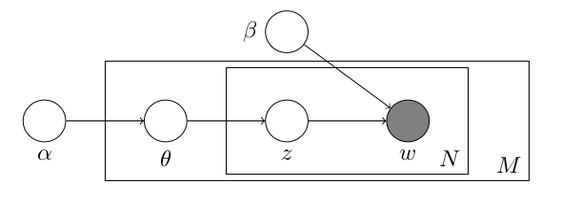
\includegraphics[width=0.6\textwidth]{figs/LDA_standard_model.png}
\caption{Plate notation of the standard LDA model}
\end{figure}
\end{center}

\paragraph{Expectation Maximization}

The Expectation Maximization, or EM, algorithm is an approach to deriving an
algorithm for approximately obtaining maximum likelihood of variables in a
statistical model. Normally one obtains a maximum likelihood solution by taking
partial derivatives of the likelihood function with respect to all variables,
setting these derivatives to zero and solving the equations simultaneously.
\cite{Myung:2003}

Due to latent variables it is not always possible to solve the equations
directly and instead one typically gets two sets of equations that depend on
each other. The EM algorithm uses the idea that one could choose starting
values for the latent variables in the first set of equations, use the result
in the second set of equations, and then alternate between the two sets until
convergence.

The general idea behind the Expectation-Maximization algorithm is this:

\begin{enumerate}
\item Start with an initial estimate of what each parameter might be.
\item \textbf{E step}: Compute the likelihood that each parameter produces 
the data point.
\item Calculate weights for each data point based on the likelihood of it 
being produced by a parameter.
\item \textbf{M step}: Combine these weights together with the data to 
compute a better estimate for the parameters.
\item Repeat steps 2 to 4 until the parameter estimate converges.
\end{enumerate}


\paragraph{Variational Inference}

In LDA, our ultimate goal is to find the posterior distribution of latent topic 
variables after observing training data. However, computing this distribution 
is intractable, so we're forced to approximate. One approximation approach is to 
use an optimization method called Variational Bayes. In the original paper it's 
being used a variational Bayes approximation of the posterior distribution;
\cite{blei2003latent} alternative inference techniques use Gibbs sampling and
expectation propagation. The goal of variational inference is to approximate an
intractable probability distribution $p$, with a tractable one $q$, in a way
that makes them as close as possible given a similarity measure. In this thesis,
variational inference is used to approximate the posterior distribution of
latent variables. A new distribution over the hidden variables $q(z, \beta)$
(called the variational distribution) is  introduced. This new distribution has
properties such that it can be efficiently computed.\cite{Fox2011ATO}

In short, we approximate the true distribution by a simple distribution $q$, and 
associate parameters $\phi$, $\gamma$, $\lambda$ with the original parameters 
$z$, $\theta$, $\beta$ respectively. Recall that $z$ gives the topic assignments 
for each word in each document, $\theta$ gives the topic composition of each 
document, and $\beta$ gives the word-topic probabilities for each word and each 
topic. The variational distribution is a function of a set of free parameters that 
are optimized such that the variational distribution is as close as possible to 
the actual target posterior distribution where closeness is measured in terms of 
KL divergence.

Specifically, we have:
\begin{equation}
q(z_{di}=k) = \phi_{dw_{di}k}
\end{equation}
\begin{equation}
q(\theta_{d}) = Dirichlet(\theta_{d}; \gamma_{d})
\end{equation}
\begin{equation}
q(\beta_{k}) = Dirichlet(\beta_{k}; \lambda_{k})
\end{equation}

The posterior over the per-word topic assignments $z$ is parametrized by
$\phi$, the posterior over per-document topic weights $\theta$ is parametrized
by $\gamma$, and the posterior over the topics $\beta$ is parametrized by
$\lambda$. 

Our goal is to estimate $\phi$, $\gamma$ and $\lambda$. In both VB and 
online VB LDA, we alternate between two steps:
\begin{enumerate}
\item E-Step: Estimate $\phi$, $\gamma$ using the current value of $\lambda$
\item M-Step: Update $\lambda$, using the current value of $\phi$
\end{enumerate}

In Variational Bayes, we perform multiple passes over the entire dataset, 
checking each time for convergence. During each pass, the algorithm does an 
E-Step using the entire dataset and an M-Step, which updates $\lambda$ using 
$\phi$ values from every document. At a high level:

\begin{algorithm}
\SetAlgoNoLine
E Step:

\For{$d = 1$ to $numDocs$}{
	initialize $\gamma$
    
    \Repeat{change in $\phi < \epsilon$}{
        update $\phi$
        update $\gamma$
     }
}
M Step:

update $\lambda$
\end{algorithm}

The specific updates are:
\begin{equation}
\phi_{d,word_{i},k} \propto e^{E_{q}(log \theta_{d,k})+E_{q}(log\beta_{k,word_{i}})}
\end{equation}
\begin{equation}
\gamma_{d,k} = \alpha + \sum_{word_{i}}\phi_{d,word_{i},k}n_{d,word_{i}}
\end{equation}
\begin{equation}
\lambda_{k,word_{i}}=\eta +\sum_{d}n_{d,word_{i}}\phi_{d,word_{i},k}
\end{equation}
Where $n_{d,word_{i}}$ is the number of occurrences of $word_{i}$ in document $d$.
The algorithm above has constant memory requirements and empirically
converges faster than collapsed Gibbs sampling. However, it still requires a
full pass through the entire corpus in each iteration. It can be slow to apply
to very large datasets.

\paragraph{Online variational LDA}


An online variational inference algorithm is proposed by Hoffman et all.\cite{onlineLDAvb} for fitting $\lambda$, the parameters to the variational
posterior over the topic distributions $\beta$. The "online LDA" is nearly as
simple as the variational algorithm, but converges much faster for large
datasets. Variational inference requires to pass through the whole dataset for
each iteration, and that can be a problem when working with big datasets and is
not an option to use cases where the data is arriving constantly. The Online
Variational Inference algorithm aims to solve both problems without compromising
the quality of the obtained topics and with an algorithm nearly as simple as
Variational Inference. For this algorithm we will only highlight the differences
respect the Variational Inference and the resulting algorithm. The key
difference is the way to fit the variational parameter $\lambda$ respect the
Variational Inference explained in the previous section.

In short, we approximate the true distribution by a simple distribution $q$, and
associate parameters $\phi,\gamma,\lambda$ with the original parameters $z,\theta,
\beta$ respectively, as in VB. Recall that $z$ gives the topic assignments for each
word in each document, $\theta$ gives the topic composition of each document, 
and $\beta$ gives the word-topic probabilities for each word and each topic.

Our goal is to estimate $\phi, \gamma, \lambda$. In both variational 
and online variational LDA, we alternate between two steps:

\begin{enumerate}
\item E-Step: Estimate $\phi, \gamma$ using the current value of $\lambda$
\item M-Step: Update $\lambda$, using the current value of $\phi$
\end{enumerate}

In online Variational Bayes, we only make a single sweep of the entire dataset, 
analyzing a chunk of documents at a time. A chunk could be a single document, 
50 documents, or even the entire dataset. Let's let a chunk be 1000 documents.

The online E-Step only uses the current chunk; instead of holding all the 
documents we now only have to hold 1000 in memory. The E-Step finds locally 
optimal values for $\phi$ and $\gamma$, while in the M-Step, we first compute 
$\lambda^{*}$, which is the value of $\lambda$ if we imagined that the entire 
dataset is made up of $\frac{numDocs}{chunkSize}$ copies of the current chunk. 
Then $\lambda$ is updated using a weighted sum of $\lambda^{*}$ and $\lambda$:

\begin{algorithm}
\SetAlgoNoLine
E Step:

initialize $\gamma$

\Repeat{change in $\phi < \epsilon$}{
        update $\phi$
        
        update $\gamma$
}
M Step:

compute $\lambda^{*}$

update $\lambda$
\end{algorithm}

We can see that unlike variational LDA, in online LDA we only need to hold a
small chunk of the data at a time, and once we're done analyzing it, we never
need it again. As with batch, once we've estimated $\lambda$, we can find the 
most probable words for each topic by looking at the word probabilities in 
each row of $\lambda$.\footnote{\url{https://wellecks.wordpress.com/2014/10/26/ldaoverflow-with-online-lda/}}

\section{Methodology}

In this section, we explain the procedure that we followed in n order to apply
the LDA model in our dataset. The dataset consists of two datasets: the one that
contains all the information about EU projects founded for research and
innovation under the FP4-H2020 and the dataset from USA about the
awards/projects that got approved from 1994-2017. We consider the projects'
description/abstract as the documents in LDA. 

\subsection{EU dataset}

CORDIS (Community Research and Development Information Service) is the European
Commission's primary public repository and portal to disseminate information on
all EU-funded research projects and their results in the broadest sense. The
website includes all public information held by the Commission (project
fact sheets, publishable reports and deliverables), editorial content to support
communication and exploitation (news, events, success stories, magazines) and
comprehensive links to external sources such as open access publications and
websites. CORDIS is managed by the Publications Office of the European Union, on
behalf of the European Commission's research Directorates-General and Agencies.
CORDIS content dates back to the origin of the service in 1990 and the website
has been online since 1994.


Below, we provide the general topics of the EU projects as listed in the EU 
Open Data Portal \footnote{https://data.europa.eu/euodp/en/data}:
\begin{itemize}
\item Agriculture, Fisheries and Food
	\begin{description}
	\item Agriculture, Food safety, Maritime affairs and fisheries
	\end{description}
\item Business
	\begin{description}
	\item Competition, Enterprise, Single market, Trade
	\end{description}
\item Culture and Education
	\begin{description}
	\item Audiovisual and media, Culture, Education training and youth, Multilingualism
	\end{description}
\item Customs and Tax
	\begin{description}
	\item Customs, Taxation
	\end{description}
\item Development and Humanitarian aid
	\begin{description}
	\item Development and cooperation, Humanitarian aid and Civil protection, Human rights
	\end{description}
\item Economy and Finance
	\begin{description}
	\item Budget, Economic and monetary affairs, Fraud prevention
	\end{description}
\item Employment and Social affairs
\item Enlargement and Foreign affairs
\item Environment and Energy
	\begin{description}
	\item Climate action, Energy, Environment
	\end{description}
\item EU institutions
	\begin{description}
	\item Institutional affairs
	\end{description}
\item Health
	\begin{description}
	\item Health, Sport
	\end{description}
\item Justice and Citizens' rights
	\begin{description}
	\item EU citizenship, Consumers, Justice and Home affairs
	\end{description}
\item Regions and Local development
	\begin{description}
	\item Regional policy
	\end{description}
\item Science and Technology
	\begin{description}
	\item Space, Digital Economy and Society, Research and Innovation
	\end{description}
\item Transport and Travel
\end{itemize}

The data that are provided by CORDIS (via the EU Open Data Portal) are open,
free and can be used in research, applications, commercial or non-commercial
purposes. The dataset that we chose for the following analysis contains
information about all the projects funded by the European Union from 1994 to
2017. These projects got approved under the framework programme (FP4-H2020) for
research and technological development. For each project it is provided
information, such as: reference, acronym, dates, funding, programs,
participant countries, subjects and objectives.

In the provided dataset, the information is splitted into CSV files, based on
the framework program that each project belongs. The frameworks from 1994 to
2020 are listed below:

\begin{itemize}
\item FP4: fourth framework programme (1994-1998)
\item FP5: fifth framework programme (1998–2002)
\item FP6: sixth framework programme (2002–2006)
\item FP7: seventh framework programme (2007–2013)
\item H2020: Horizon 2020 framework programme (2014-2020)
\end{itemize}

\subparagraph{Data preparation}

Data cleaning is absolutely crucial for generating a useful topic model. 
We implemented the following steps, which are common to most natural 
language processing methods, in order to obtain the final corpus for the 
analysis:

\begin{itemize}
\item Remove punctuation and numbers
\item Tokenize documents
\item Remove stopwords
\item Create a dictionary
\item Filter out the most frequent and some rare words of the dictionary
\end{itemize}

To obtain the collection of the documents, we consider as 'documents' in LDA the
project objectives, which is an accurate description for the project. We also
added the 'title' value of each project to the objectives-documents, to increase
the probability of finding accurate topics. For the majority of the projects the
'start date' and 'end date' value was null, so we kept the splitting of the
dataset per framework, in order to keep the correlation to the time. We followed
the same format in the dataset of USA awards.


\begin{center}
\begin{tabular}{l*{6}{c}r}
Framework & Years & No of docs & No of unique tokens & No of words in the corpus \\
\hline
FP4 & 1994-1998 & 14567 & 7293 & 364263 \\
FP5 & 1998-2002 & 17202 & 15756 & 1617232 \\
FP6 & 2002-2006 & 10091 & 15521 & 1437607 \\
FP7 & 2007-2013 & 25607 & 26499 & 3789837 \\
H2020 & 2014-2017 & 9055 & 15835 & 1342882 \\
\end{tabular}
\end{center}

As stopwords, we used the list that is provided by the Gensim Python
library\footnote{http://radimrehurek.com/gensim/} and we added following very
common words in the existing dataset: 'data', 'based', 'new', 'project',
'university', 'student', 'students', 'research', 'study', 'program',
'development', 'study', 'studies', 'provide', 'use'. We also removed the rare
words that appear less than 5 times in the collection. Finally, we obtained a
smaller corpus per framework (see the table above)

In this section, we explain the procedure that we followed in n order to apply
the LDA model in our dataset. The dataset consists of two datasets: the one that
contains all the information about EU projects founded for research and
innovation under the FP4-H2020 and the dataset from USA about the
awards/projects that got approved from 1994-2017. We consider the projects'
description/abstract as the documents in LDA. 

\subsection{USA dataset}

The National Science Foundation (NSF) is a United States government agency that
supports fundamental research and education in all the non-medical fields of
science and engineering. Its medical counterpart is the National Institutes of
Health. The NSF funds approximately 24\% of all federally supported basic
research conducted by the United States' colleges and universities. In some
fields, such as mathematics, computer science, economics, and the social
sciences, the NSF is the major source of federal backing.

 
The NSF organizes its research and education support through seven 
directorates, each encompassing several disciplines:

\begin{itemize}
\item Biological Sciences
\begin{description}
\item Molecular, Cellular and Organismal biology, Environmental science
\end{description}
\item Computer and Information Science and Engineering
\begin{description}
\item Fundamental computer science, Computer and networking systems, 
Artificial Intelligence
\end{description}
\item Engineering
\begin{description}
\item Bioengineering, Environmental systems, Civil and Mechanical systems, 
Chemical and Transport systems, Electrical and Communications systems, Design
 and Manufacturing
\end{description}
\item Geosciences
\begin{description}
\item Geological, Atmospheric and Ocean sciences
\end{description}
\item Mathematical and Physical Sciences
\begin{description}
\item Mathematics, Astronomy, Physics, Chemistry and Materials science
\end{description}
\item Social, Behavioral and Economic Sciences
\begin{description}
\item Neuroscience, Management, Psychology, Sociology, Anthropology, 
Linguistics, Science of science policy and economics
\end{description}
\item Education and Human Resources
\begin{description}
\item Science, Technology, Engineering and mathematics education at every level
\end{description}
\end{itemize}

The data about the awards
\footnote{https://www.nsf.gov/awardsearch/download.jsp} are open, free and can
be used in research and applications. The dataset that we chose for the
following analysis contains information about all the projects that got funded
by the NSF from 1994 to 2017.
 
In the provided dataset, the information is splitted into XML files, separated
per year, from 1994 - 2017. In order to keep the correlation to time and be able
to compare the two datasets later, we splitted the projects based on the year
they were initialized (see Table below).


\subparagraph{Data preparation}

Just like the EU dataset, we followed the same preprocessing steps to obtain the
final corpus. As stopwords, we used the list that is provided by the Gensim
Python library and we removed following very common words in the existing
dataset: 'data', 'work', 'based', 'new', 'project', 'university', 'student',
'students', 'research', 'study', 'program', 'development', 'study', 'studies',
'provide', 'use', 'understanding', 'important', 'support', 'proposed'. We also
removed the rare words that appear less than 5 times in the collection. Finally,
we obtained a smaller corpus per framework (see Table below).

\begin{center}
\begin{tabular}{l*{6}{c}r}
Framework& Years & No of docs & No of unique tokens & No of words in the corpus \\
\hline
FP4 & 1994-1997 & 36752 & 28038 & 4346604 \\
FP5 & 1998-2001 & 37674 & 30728 & 5166316 \\
FP6 & 2002-2006 & 54212 & 38476 & 8837298 \\
FP7 & 2007-2013 & 87341 & 48277 & 15673424 \\
H2020 & 2014-2017 & 35581 & 32268 & 7379219 \\
\end{tabular}
\end{center}

\subsection{Model inference}

For the implementation, we used the Gensim package (Radim Řehůřek,
2009)\cite{rehurek_lrec} which implements an efficient online LDA algorithm, to
extract the topics of a given corpus. Gensim uses a fast implementation of
online LDA parameter estimation based on "Online Learning for Latent Dirichlet
Allocation".\cite{onlineLDAvb} The algorithm runs in constant memory, which
means that the size of the training corpus does not affect memory footprint, so
it can process corpus larger than RAM.

The LDA model requires some basic input parameters; for both datasets we chose
the number of topics $K=10$. The hyper-parameter $\alpha$, which affects the
sparsity of the document-topic distribution $\theta$, is by default a symmetric
$\frac{1.0}{num_topics} = 0.1$ prior. We left the default value of $chunksize=2000$. We
started with 50 iterations and later we increased the number of iterations,
until the training converged. We used 7000 iterations for each framework
programme of the EU dataset and 8000 for each framework of the USA dataset. In
the USA dataset, we used $passes=1$, while in the EU dataset we switched to
$passes=2$, because the training could not converge, despite the large number of
the iterations.

The implementation was run on a computer with an Intel® Xeon® Processor E5-1410
(10MB Cache, 2.8 GHz, 4 cores, 8 threads) and RAM=12 GB. Check the Appendix for 
the actual implementation.


\section{Analysis and results}

In this section, we show our main results. We focus on finding differences
between the two datasets in terms of topic distribution and later we 
investigate the evolution of the topics over time of each dataset separately.


\subsection{Discovering topics on the EU projects}

In general, the most popular subject in European Union over the years is
Information systems. In our dataset we fount projects related to almost all
kinds of information systems, and especially Quality management systems
(1994-2002), Management information systems, Network information systems and
Information systems as a service to all kinds of organizations, including
universities and companies. Since technology has an impact in every aspect
nowadays, it is normal to have such popularity over the years and it's becoming
popular in education, as well. The same period of time, Innovation in Business
emerged as a trending topic, with projects related to new technologies and
software systems in the industry and how they assist the businesses and the
market. In addition, until 2002 a very popular subject related to Information
systems, was Applications in mobile networks, embedded and broadband systems,
which nowadays has lost part of its popularity in research.

Another popular subject that appears the last 22 years is Materials research;
the projects related to material research are mostly related to the discovery
and design of new materials, with an emphasis on solids. Materials properties
and performance are used in many disciplines, like chemistry, physics and
engineering.

The third most popular subject is Molecular biology and Genetics. These projects
are related to the cellular molecules that carry out the biological processes
essential for the cell's functions and maintenance. These affect many aspects of
our lives, including evolution, nutrition and the spread of diseases. Especially
from 1998 up to day, there is a focus in Health care and Diagnostics, and for the
last decade researchers are studying the cancer detection and treatment, which
is a common cause of death in EU and the second most common cause of death in
USA.

Moreover, Environmental, Social and Economic Sustainability is a subject very
important to the research community and many researchers work on this up to day.
In short, sustainability takes into account how we might live in harmony with
the natural world around us, protecting it from damage and destruction. Many
projects are related to one of the Three Pillars of Sustainability\footnote{http
://www.thwink.org/sustain/glossary/ThreePillarsOfSustainability.htm}. The
European Union is considered by some to have the most extensive environmental
laws of any international organization, started by the  European Economic
Community (EEC), which is the beginning of the EU's environmental policy. Social
and Economic policies are also popular in the EU region over the last decade.
Also, the last two decades there is a focus on the Green energy production, like
hydropower, solar and nuclear energy.

During the 6th and the 7th framework programme, International Research and
conferences came up in our dataset as a trending topic. Researchers have a great
interest to collaborate with other colleagues from all over the world and share
their knowledge. A big part of the projects funded by the EU that is related to
international research, is also related to Physics, in general, and High energy
physics in EU (see Appendix: Wordclouds of topics of the EU).

\subsection{Discovering topics on the USA projects}

The National Science Foundation mostly supports fundamental research and
education in the non-medical science and engineering. Its medical counterpart
is the National Institutes of Health.\footnote{\url{https://en.wikipedia.org/wik
i/National_Science_Foundation}} With STEM being the top priority in USA, most of
the projects founded by NSF are related to engineering, computer science,
mathematics and information systems, in general. The subjects STEM \& Education,
Software engineering, Information systems and Mathematics, arise as topics in
all these years, from 1994-2017.

While NSF promotes the progress of science, it also enhances the efforts to
maintain the national health, prosperity, and welfare. Over the last 22 years,
many projects are related to the environment effects of climate change. Topics
like Environmental Science, Atmospheric \& Ocean sciences, Geology, Climate
change and its impact in the United States emerge during all these years. The
last three years there is a focus on the Green energy production, like
hydropower and wind power. Among with climate change, there is many research
related to Biology and Evolution. A less popular subject that appears during the
years 1994-1997 and 2007-2013 is Molecular, Cellular \& Organismal biology and
Genetics. These projects mostly refer to applied genetics, as well as cell
functionality. Topics include receptor biology, regulation of gene expression,
biomedical engineering, patterns of inheritance and molecular genetics.

Another popular subject that appears the last 22 years is Materials and
Chemistry; the projects related to material research are mostly refer to the
materials' properties and applications in engineering. The last 3 years,
researchers from the USA focus on materials applications and design in
mechanical engineering, bioengineering and chemical \& transport systems. In
2002-2006 many projects are related to the subject of transport that is
sustainable in the senses of social, environmental and climate impacts (Green
transportation).

From 1994-2006 and the last three years, International Research and conferences
came up as a trending topic. Re- searchers have a great interest to collaborate
with other colleagues from all over the world and share their knowledge. A big
part of the projects funded by the EU that is related to international research,
is also related to Physics, in general, and High energy physics in EU (see
Appendix: Wordclouds of topics of the EU).

NSF shows a great interest in international activities across all NSF supported
disciplines. The goal of these projects is to support high quality research and
education, which could not occur without international collaboration. NSF seeks
to catalyze a higher level of international engagement in the U.S. science and
engineering community by promoting International conferences and university
projects and partnerships. An interesting fact regarding international
partnerships is that the European Commission and the Government of the United
States of America concluded on 17 October 2016 an Implementing Arrangement that
simplifies the cooperation between Horizon 2020 projects and US entities.
European and American researchers will be able to work together more closely on
projects funded under Horizon 2020, the European Union's research and innovation
programme.\footnote{\url{http://ec.europa.eu/research/iscp/index.cfm?pg=usa}}

From 2002 up to day, Economic and Social Sciences emerge as a topic in our
dataset. Researchers show a great interest in identifying policies which help
the communities and they also do lots of Qualitative and Quantitative research
to investigate the size or extent of particular issues or trends in society.

Finally, a topic that used to be popular in the past, in 1994-1997 and
2007-2013, is High energy Physics in USA, which has lost its popularity
nowadays. The last 5 years, there is an interest around STEM and its
applications in manufacturing and engineering.


\subsection{Topic evolution over time}

One of our goals is to identify trends in scientific research in EU and USA, in
order to give some insights to researchers and scientists regarding potential
trends. For this analysis, we run the model for the whole dataset, instead of
running the model per FP), for the EU and the USA, respectively. The outcome was
10 topics for each region from 1994 to 2017 for the EU and from 1994 to 2016 for
the USA.\footnote{in this implementation we removed the projects of the year
2017 from the USA dataset, because the amount of projects-documents was too
small compared to the other years and it was affecting the result of the trend
for each topic.}

\subparagraph{Trends in the EU}

In figure x we show the 10 topics that consists of the 20 top words with the
highest posterior probability of belonging to the topic. The size of each word
is in proportion to each probability; the bigger the word, the higher the
probability. Each wordcloud describes a topic, which we can find intuitively.
Below are listed the topics that we found corresponding to the words that
describe them:
\begin{itemize}
\item[] Topic 0: Molecular biology
\item[] Topic 1: Materials \& Manufacturing
\item[] Topic 2: Social policy
\item[] Topic 3: Disease detection \& treatment
\item[] Topic 4: Materials science / Physics
\item[] Topic 5: Transport \& Energy
\item[] Topic 6: Business \& Innovation
\item[] Topic 7: Climate change / Environment
\item[] Topic 8: Molecular mechanisms
\item[] Topic 9: Information systems
\item[] Topic 10: International research
\item[] Topic 11: Energy production
\end{itemize}
\begin{center}
\begin{figure}
\begin{tabular}{rcl}
\subfloat[Topic 0]{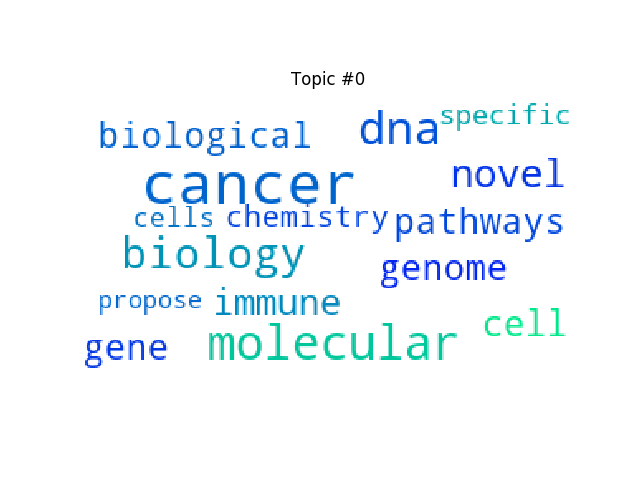
\includegraphics[width=0.35\textwidth]{figs/eu_topics/EU_topic0_all.png}} &
\subfloat[Topic 1]{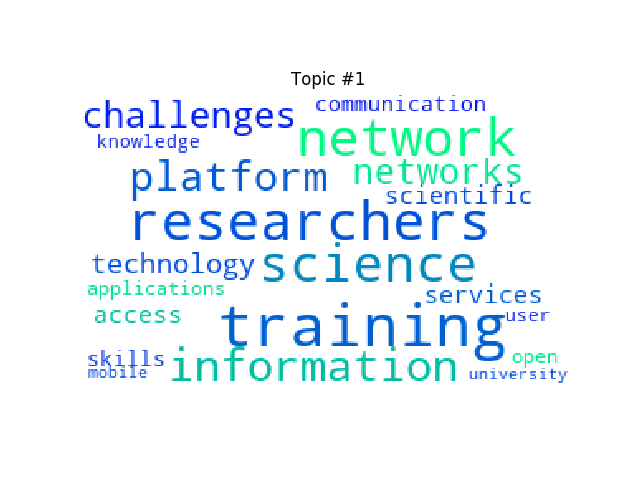
\includegraphics[width=0.35\textwidth]{figs/eu_topics/EU_topic1_all.png}} &
\subfloat[Topic 2]{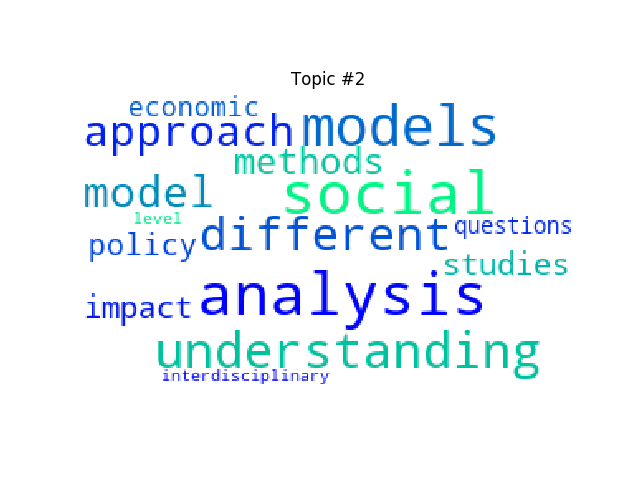
\includegraphics[width=0.35\textwidth]{figs/eu_topics/EU_topic2_all.png}}\\
\subfloat[Topic 3]{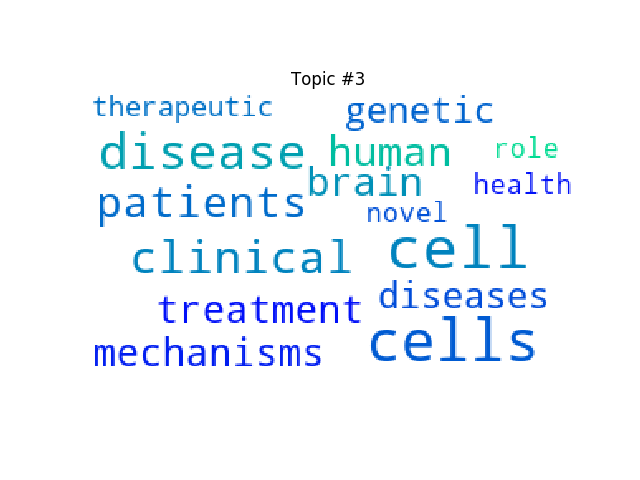
\includegraphics[width=0.35\textwidth]{figs/eu_topics/EU_topic3_all.png}} &
\subfloat[Topic 4]{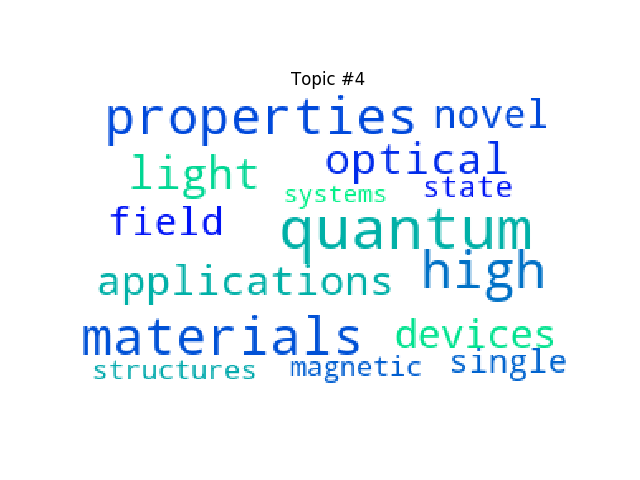
\includegraphics[width=0.35\textwidth]{figs/eu_topics/EU_topic4_all.png}} &
\subfloat[Topic 5]{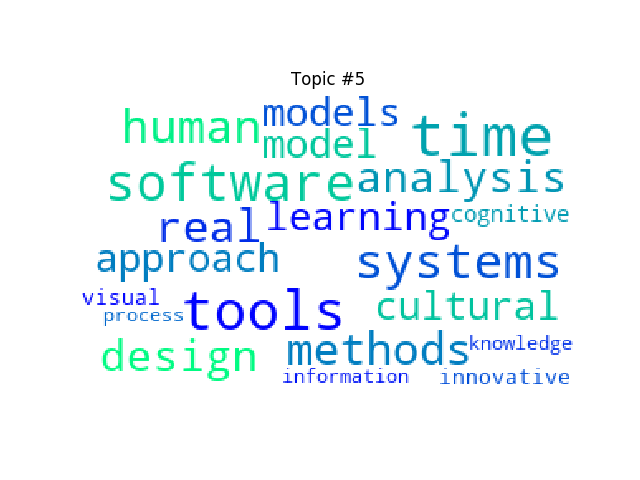
\includegraphics[width=0.35\textwidth]{figs/eu_topics/EU_topic5_all.png}}\\
\subfloat[Topic 6]{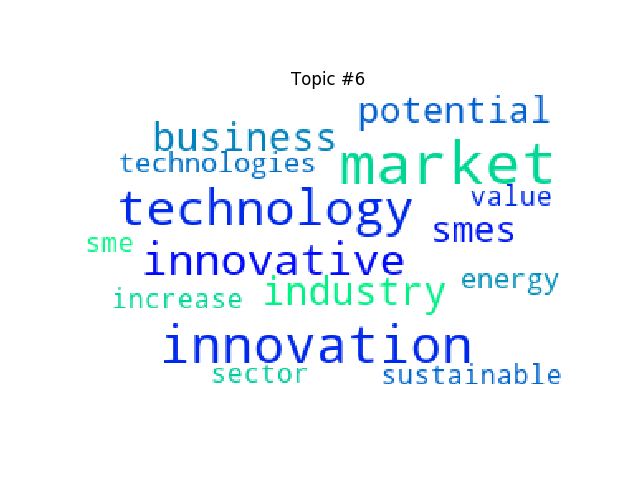
\includegraphics[width=0.35\textwidth]{figs/eu_topics/EU_topic6_all.png}} &
\subfloat[Topic 7]{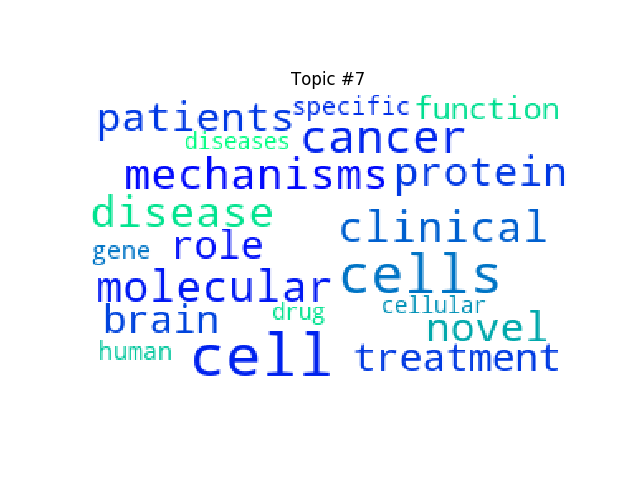
\includegraphics[width=0.35\textwidth]{figs/eu_topics/EU_topic7_all.png}} &
\subfloat[Topic 8]{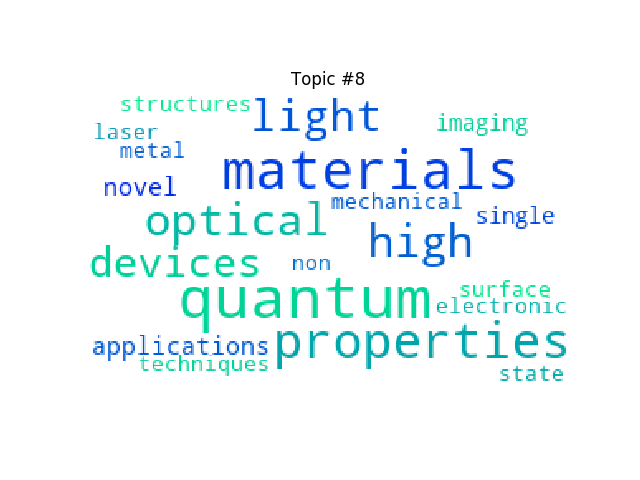
\includegraphics[width=0.35\textwidth]{figs/eu_topics/EU_topic8_all.png}}\\
\subfloat[Topic 9]{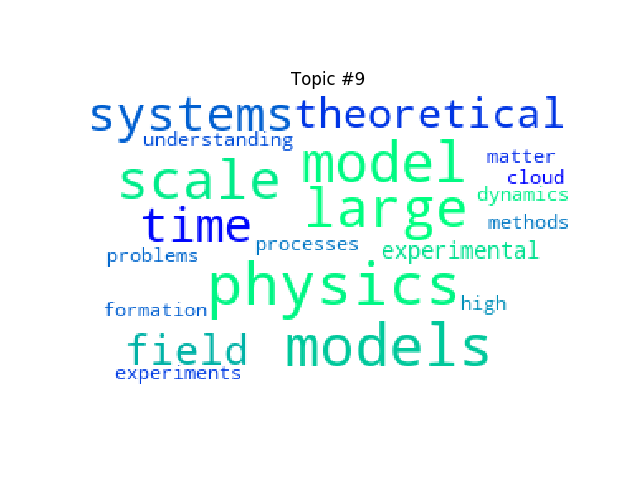
\includegraphics[width=0.35\textwidth]{figs/eu_topics/EU_topic9_all.png}} &
\subfloat[Topic 10]{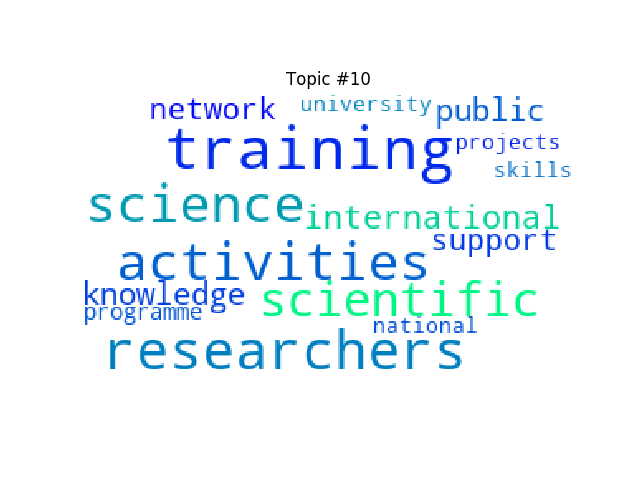
\includegraphics[width=0.35\textwidth]{figs/eu_topics/EU_topic10_all.png}} &
\subfloat[Topic 11]{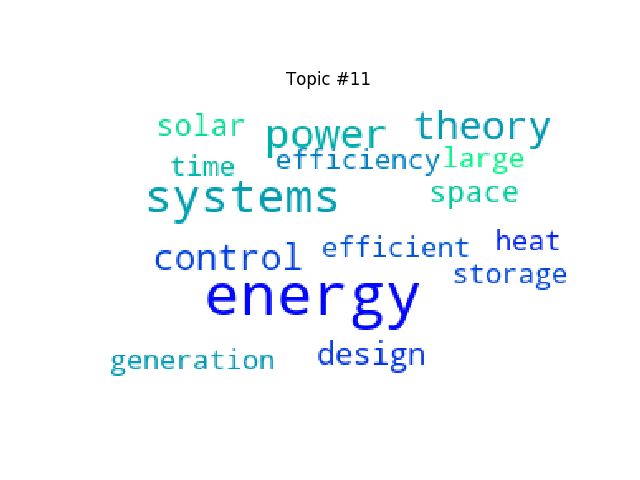
\includegraphics[width=0.35\textwidth]{figs/eu_topics/EU_topic11_all.png}}\\
\end{tabular}
\caption{Wordclouds of topics of the EU dataset (1994-2017)}
\end{figure}
\end{center}
In order to find the topic distribution over time, we need the topic
distribution of each project-document. As we mentioned before, LDA assumes that
each document exhibits multiple topics. After running the model to our dataset,
we get the document-topic distribution and we keep the topic with the highest
probability (the one that most likely belongs to this document). Then, we
calculate the proportion of each topic per FP, using the following equation:
\begin{equation}
topicProportion(k, fp) = \frac{\sum num of docs_{k,fp}}{\sum num of docs_{fp}} * 100
\end{equation}
where $k$ is the number of the topic id, $fp$ is the framework programme,
$fp \in [FP4, FP5, FP6, FP7, H2020]$. The topic proportion of each topic in 
the FP equals to the sum of the number of the documents assigned to this 
topic during the FP, normalized by the number of the documents-projects 
occurring in this FP. In figure X we plot the results of the topic proportion 
over time.

Based on this plot, topic 10, which refers to International Research, has an
interesting evolution; During the years 1994-1998 is appears as less popular
topic, compared to other topics. However, this state changes drastically in
1998-2002 ($+14\%$) and in 2002-2006 it is at its peak ($+18\% since 1994$).
This period many activities and projects where initialized in order to support
and promote international education and conferences to attract researchers from
all over the world. Strangely, this trend has a significant decrease the last 10
years, compared to other topics ($-12\%$). We already know that in Horizon 2020
there is an agreement between EU and USA for supporting the cooperation of the
two regions.Our hypothesis for the evolution of the International Research is
that the EU successfully managed to create the foundation for supporting
international people and there is no need to invest more on projects that
attempt to promote cooperation between international researchers, because it is
already considered as a common practice nowadays.

Materials and Manufacturing was a hot topic in 1994-1998, but it also appears a
big decrease during the years 1998-2006 and it has a stable trend since then.
Materials Science/Chemistry \& Physics' popularity (topic 4) line has an
increase during 2002-2013 and the last 3 years a small decrease of $2-3\%$.
Topics 2 and 3 (Social policy, Disease detection \& treatment) follow the same
linear trend as Materials science \& Physics. Energy production (topic 11) was
less popular in 1994-2002 and is becoming slightly popular the last 15 years.

Topic 9, which refers to Information systems in general, is a subject that has a
stable trend and it appears as a popular topic the last 22 years compared to
other topics, with a percentage of $12.5\%$ of the projects in EU on average.

Biology and the study of molecular mechanisms have a small decrease of
popularity on average. This may happen because the projects related to medical
fields are supported by another institute, National Institutes of Health. Also,
research in Climate change and Environmental science is another subject that
paradoxically appears as a topic that is gradually losing its popularity over
the last years.

Finally, topic 6, which is related to Business \& Innovation, has a huge
increase the last 3 years. We can assume that the EU is very interested in
supporting the economy by funding projects about businesses and monetary
affairs.
\begin{center}
\begin{figure}
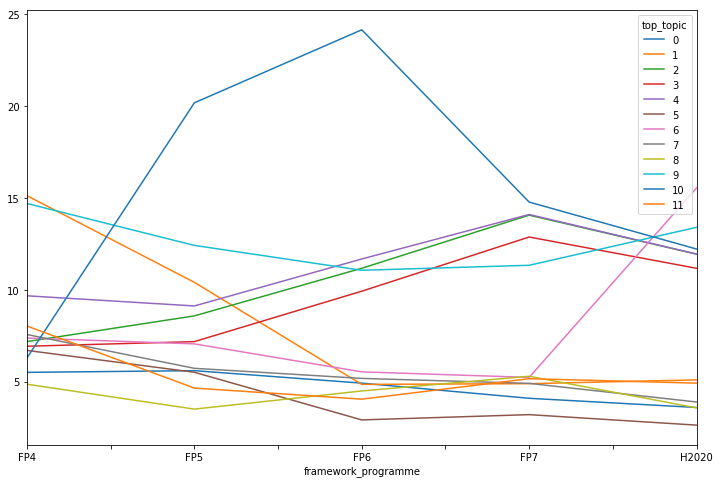
\includegraphics[width=1.0\textwidth]
{figs/eu-topic-evolution.png}
\caption{Topics over time in EU}
\end{figure}
\end{center}
\subparagraph{Trends in the USA	}

Just like the EU dataset, we found the 10 topics of the USA dataset from 1994 to
2016. Since, we're looking for the topic distribution over time, in this
implementation we took the projects per year (instead of using the separation of
the dataset per FP), to visualize the evolution of each topic per year. We ran
the LDA model with 12000 iterations and the dame value of the rest of the
parameters, as described in section 4.3.

Each one of the wordclouds in figure X represents a topic. The topics that are
described in the wordclouds are listed below:

\begin{itemize}
\item[] Topic 0: Material science and High energy physics
\item[] Topic 1: Mathematics
\item[] Topic 2: (Molecular) biology, Genetics
\item[] Topic 3: Science of social policy and economics
\item[] Topic 4: International research and conferences
\item[] Topic 5: Chemistry and Materials science
\item[] Topic 6: STEM education
\item[] Topic 7: Climatology, Atmospheric and Ocean sciences
\item[] Topic 8: Molecular biology 
\item[] Topic 9: Mechanical engineering
\end{itemize}

\begin{center}
\begin{figure}
\centering
\begin{tabular}{rcl}
\subfloat[Topic 0]{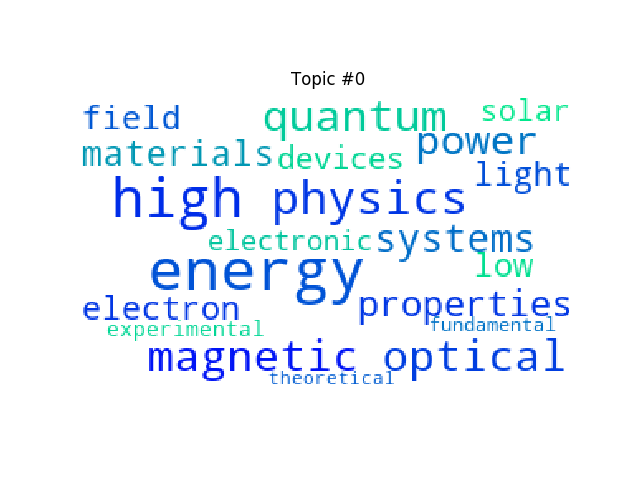
\includegraphics[width=0.35\textwidth]{figs/usa_topics/USA_topic0_12000_all_docs.png}} &
\subfloat[Topic 1]{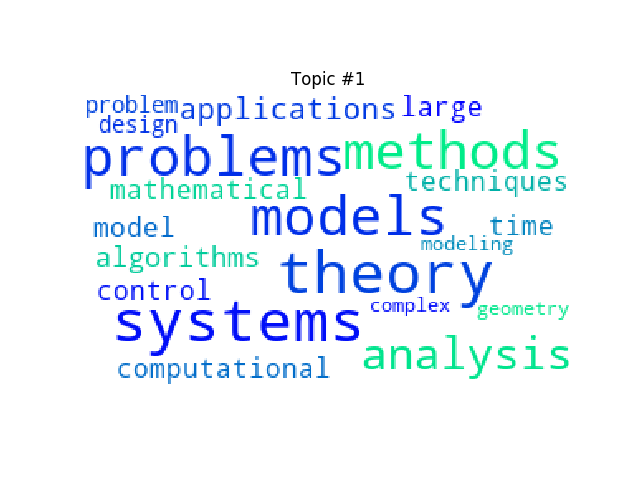
\includegraphics[width=0.35\textwidth]{figs/usa_topics/USA_topic1_12000_all_docs.png}} &
\subfloat[Topic 2]{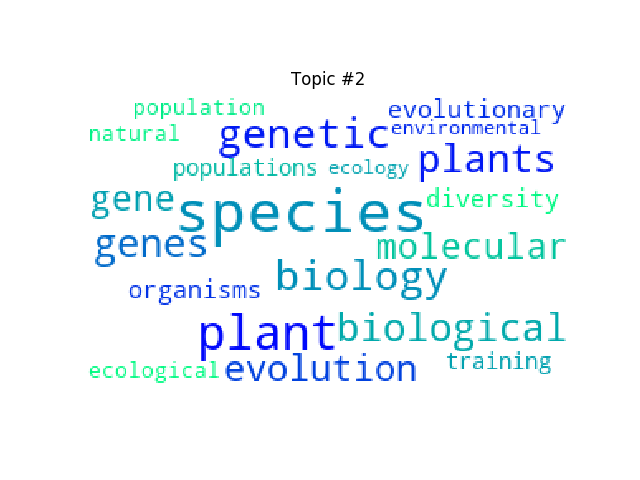
\includegraphics[width=0.35\textwidth]{figs/usa_topics/USA_topic2_12000_all_docs.png}}\\
\subfloat[Topic 3]{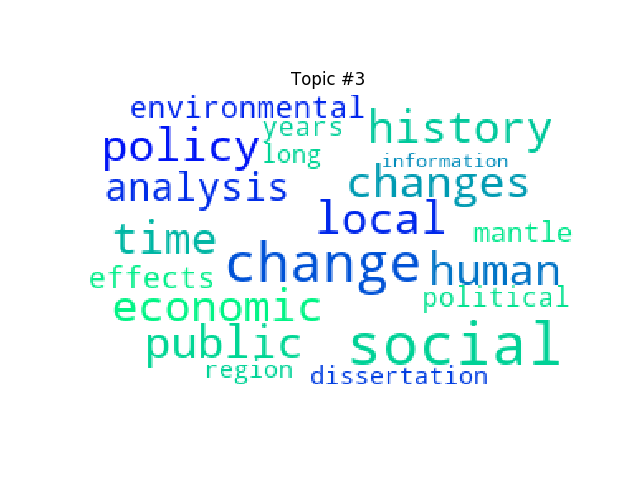
\includegraphics[width=0.35\textwidth]{figs/usa_topics/USA_topic3_12000_all_docs.png}} &
\subfloat[Topic 4]{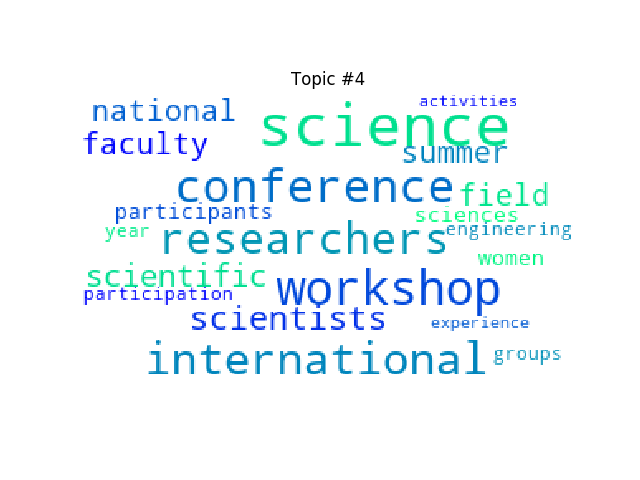
\includegraphics[width=0.35\textwidth]{figs/usa_topics/USA_topic4_12000_all_docs.png}} &
\subfloat[Topic 5]{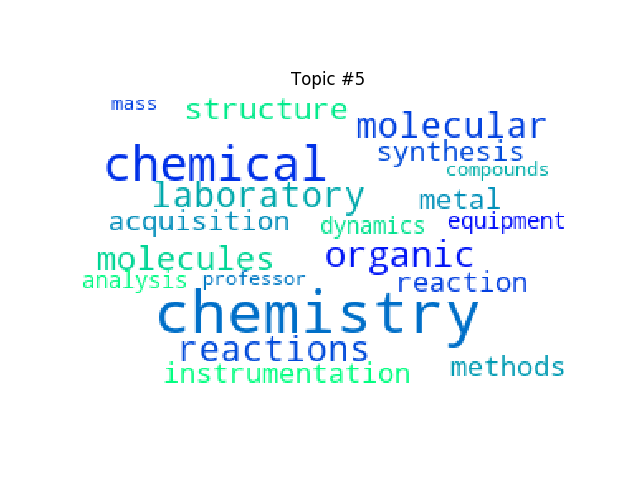
\includegraphics[width=0.35\textwidth]{figs/usa_topics/USA_topic5_12000_all_docs.png}}\\
\subfloat[Topic 6]{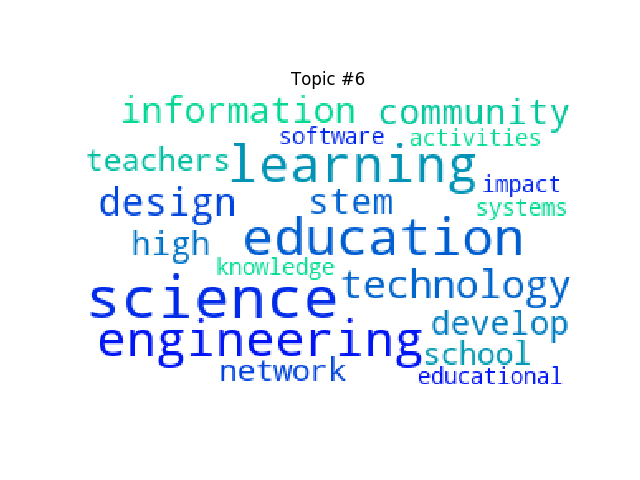
\includegraphics[width=0.35\textwidth]{figs/usa_topics/USA_topic6_12000_all_docs.png}} &
\subfloat[Topic 7]{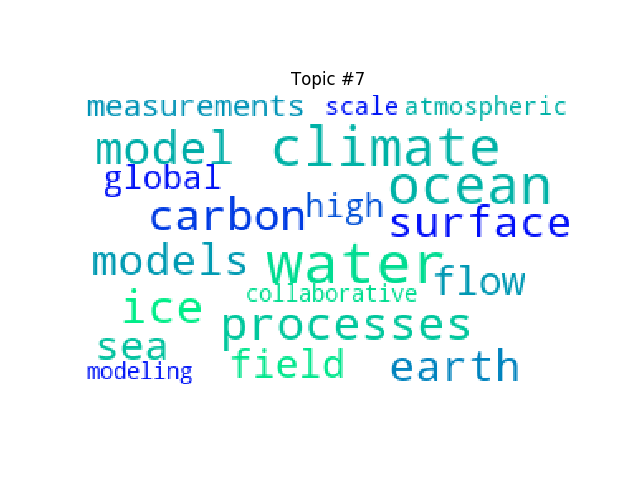
\includegraphics[width=0.35\textwidth]{figs/usa_topics/USA_topic7_12000_all_docs.png}} &
\subfloat[Topic 8]{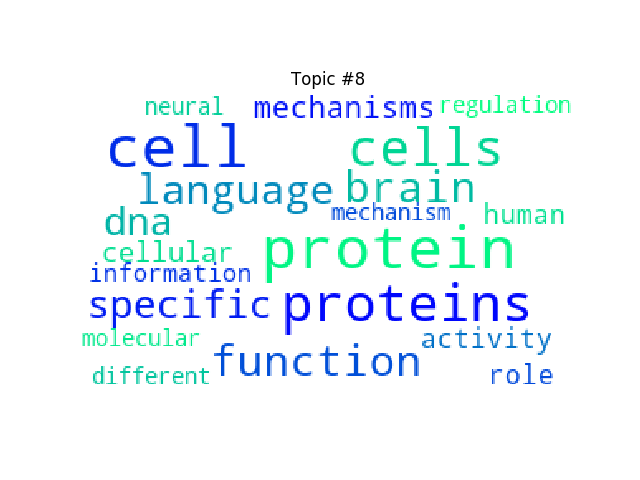
\includegraphics[width=0.35\textwidth]{figs/usa_topics/USA_topic8_12000_all_docs.png}}\\
\subfloat[Topic 9]{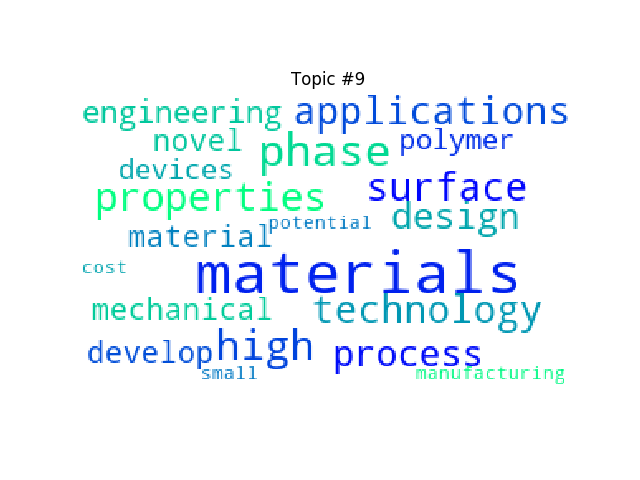
\includegraphics[width=0.35\textwidth]{figs/usa_topics/USA_topic9_12000_all_docs.png}} &
\end{tabular}
\caption{Wordclouds of topics of the USA dataset (1994-2016)}
\end{figure}
\end{center}

Just like the computation in the EU dataset, we calculate the topic 
distribution over time for the USA dataset. We get the document-topic 
distribution, we keep the topic with the highest probability and finally 
we calculate the proportion of each topic per
year (instead of FP), using the following equation:

\begin{equation}
topicProportion(k, y) = \frac{\sum num of docs_{k,y}}{\sum num of docs_{y}} * 100
\end{equation}

where $k$ is the number of the topic id, $y$ is the year between 1994-2016. The
topic proportion of each topic per year equals to the sum of the number of the
documents assigned to this topic during the year, normalized by the number of
the documents-projects  occurring in this year.

In figure X we plot the topic distribution over time. We can easily observe that
the topic 6, which refers to STEM education, is becoming a trend in the United
States over the years, while most of the other topics' evolution doesn't show up
such a high increase. Topics 5 and 8, which refer to Chemistry \& Materials
science and Molecular biology, respectively, show a small decrease over the
years. Topics 9 and 0 (Mechanical Engineering, Material Science and High energy
physics) show a small increase over the last 5 years. Mathematics' evolution
over time (Topic 1) looks stable on average and shows up as a popular subject
over the last 22 years, while Social Sciences and International Research (Topic
3 and 4) show a small decrease over the last 3 years.  Molecular biology and
Genetics (Topic 2) has an increasing popularity from 1994 to 2001 and later is
starting to stabilize. Climatology, Atmospheric and Ocean sciences look stable
the first years, while from 2006 up to date it is gradually becoming less
popular over the years.

In general, the STEM (science, technology, engineering and math) related
research and education is becoming more and more popular, which is not
surprising, since the National Science Foundation itself estimates that 80/% of
the jobs available during the next decade will require math and science skills.
Even the concept of STEM was first introduced by Judith A. Ramaley, the former
director of the National Science Foundation's education and human resources
division.
\begin{center}
\begin{figure}
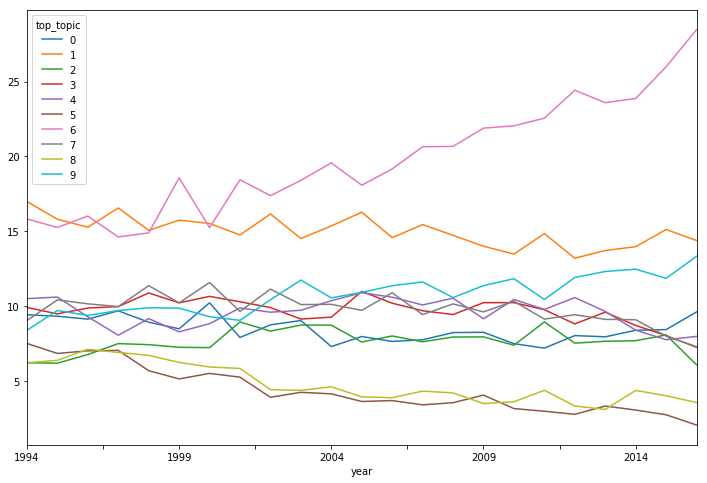
\includegraphics[width=1.0\textwidth]
{figs/topic-evolution-usa.png}
\caption{Topics over time in USA}
\end{figure}
\end{center}

\subsection{Comparison of the two regions per framework programme}

\begin{figure}
\centering
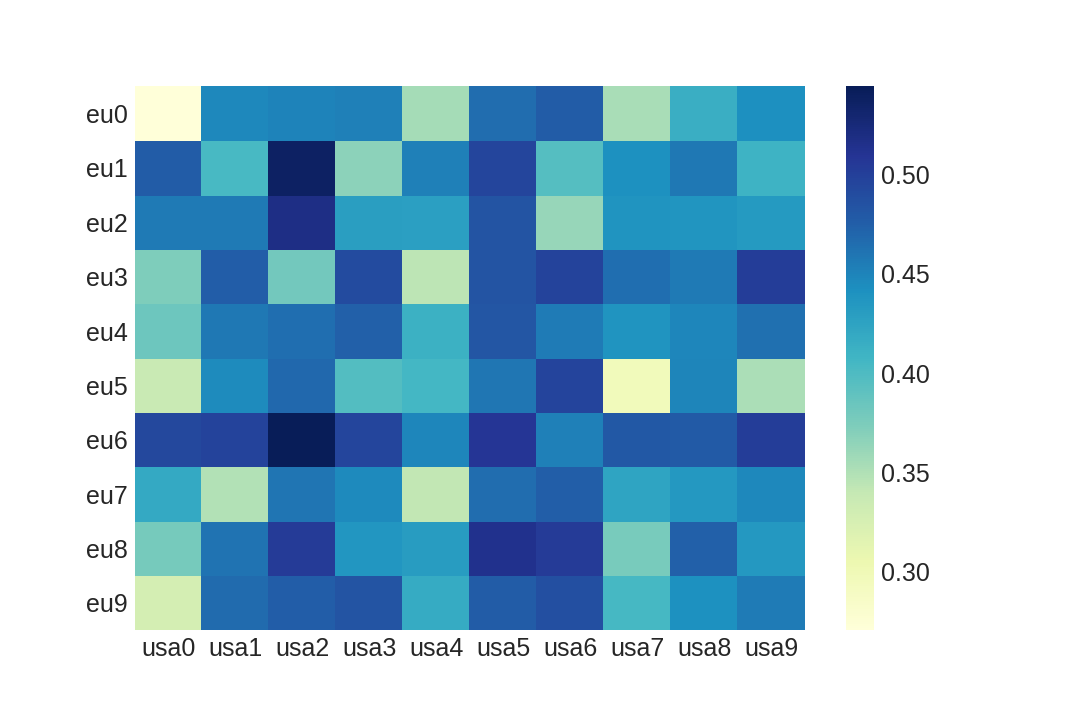
\includegraphics[width=0.8\textwidth]
{figs/heatmaps/heatmapFP4.png}
\caption{Heatmap of the similarity of the two regions during 1994-1997}
\end{figure}
\begin{figure}
\centering
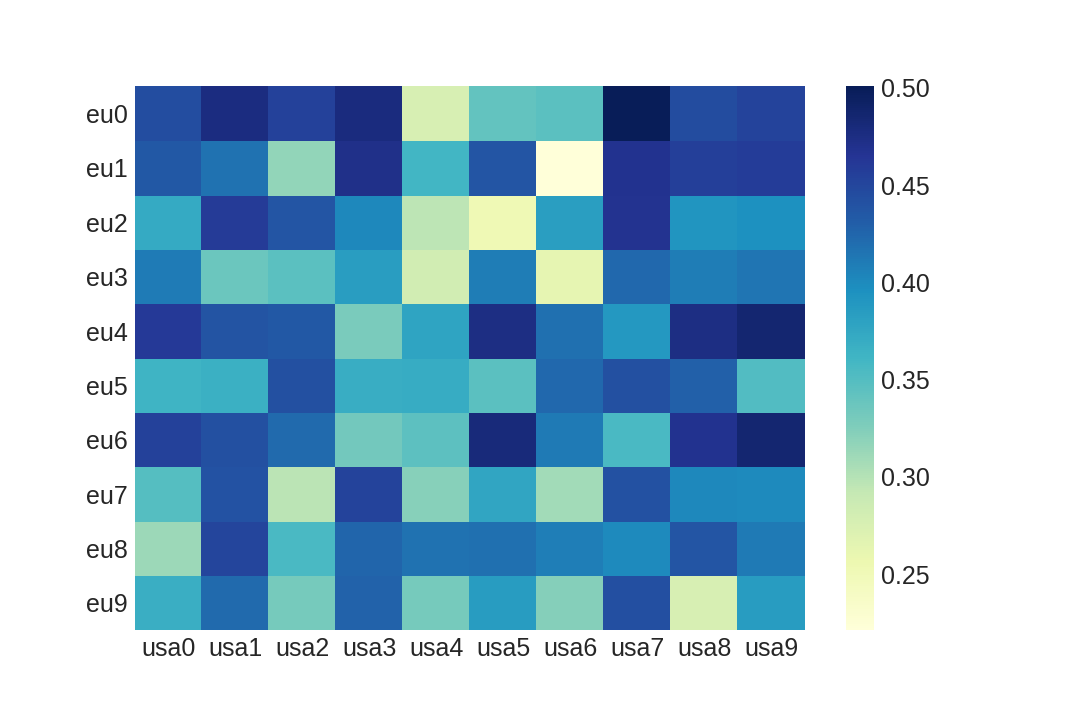
\includegraphics[width=0.8\textwidth]
{figs/heatmaps/heatmapFP5.png}
\caption{Heatmap of the similarity of the two regions during 1998-2001}
\end{figure}
\begin{figure}
\centering
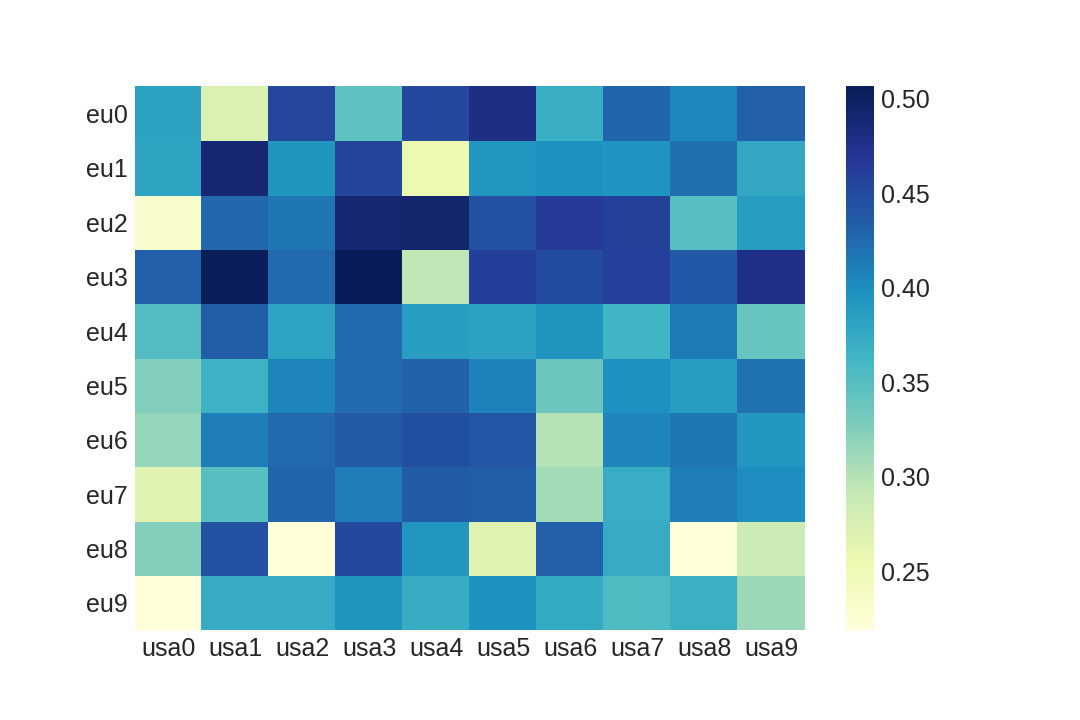
\includegraphics[width=0.8\textwidth]
{figs/heatmaps/heatmapFP6.png}
\caption{Heatmap of the similarity of the two regions during 2002-2006}
\end{figure}
\begin{figure}
\centering
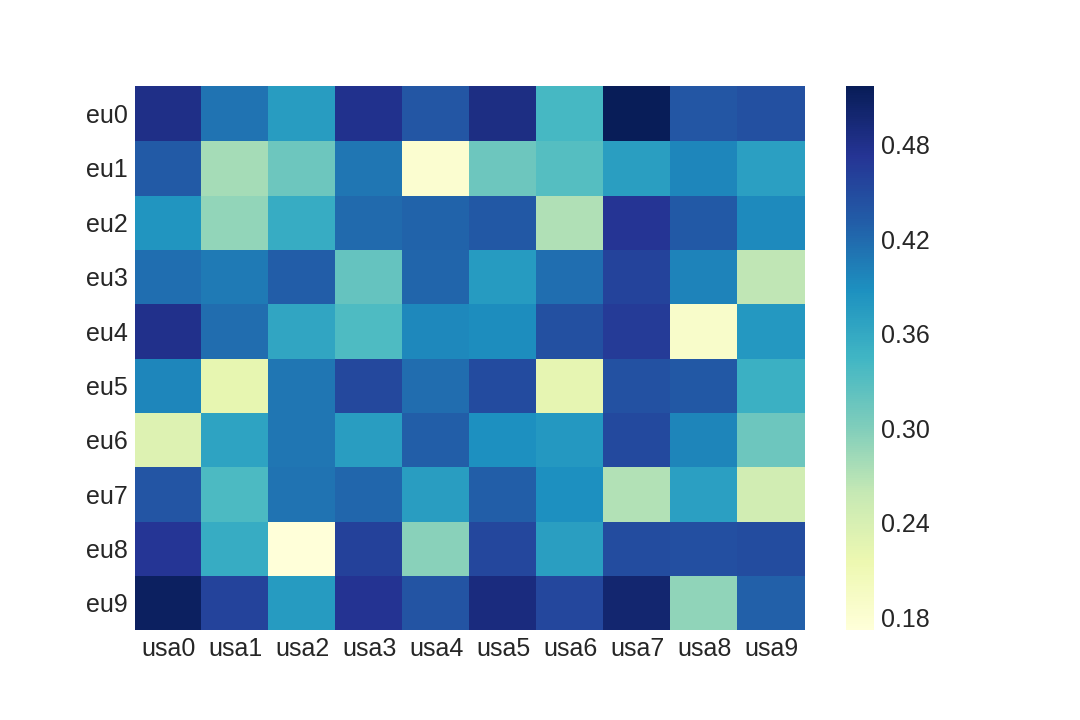
\includegraphics[width=0.8\textwidth]
{figs/heatmaps/heatmapFP7.png}
\caption{Heatmap of the similarity of the two regions during 2007-2013}
\end{figure}
\begin{figure}
\centering
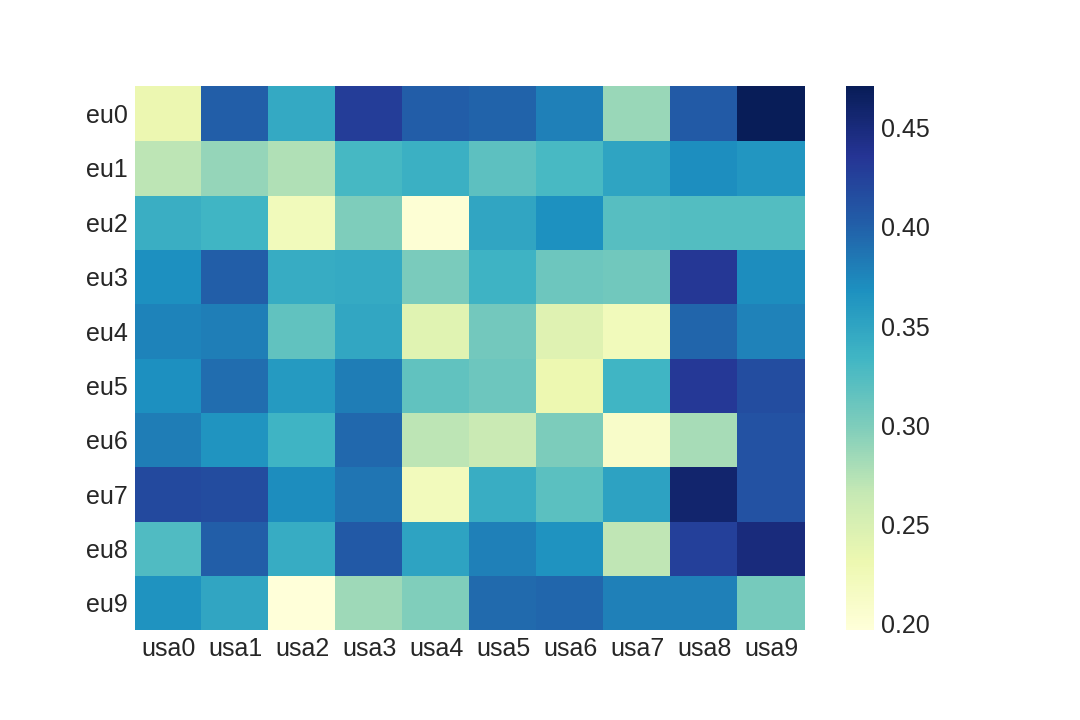
\includegraphics[width=0.8\textwidth]
{figs/heatmaps/heatmapH2020.png}
\caption{Heatmap of the similarity of the two regions during 2014-2017}
\end{figure}

\section{Conclusion}

In this thesis, we have presented a work about discovering topics and their
trends in the field of scientific research. We applied the LDA model in projects
that got funded under the European Union Framework Programmes and the projects
funded by the National Science Foundation in the United States, for research and
innovation.

We briefly describe the preprocessing of the abstracts-documents before applying
the model. LDA, as an unsupervised learning algorithm, does not require any
prior annotation of labeling the documents and the topics are resulted from the
statistical structure of the words in the corpus. Using the posterior document-
topic and topic-word distribution, we investigate the context of each topic per
FP and the evolution of the topics in each of the two datasets over time.

We found that most topics cover various topics, while some show well-defined
scopes. Our work provides valuable knowledge about the research over the last
two decades in the two regions and could benefit researchers to to identify the
subjects that mostly get funded in the EU and USA. This research gives an
interesting aspect about what kind of topics were actually funded over the last
22 years.

The results of our research have several interesting insights that can make it
easier for people to understand the information contained in large datasets,
including extracting topics and their dynamics. The evolution of the topics over
time can also help researchers to find a set of promising topics to focus on and
start a project based on this knowledge. This could potentially increase their
chances to get a funding and have the opportunity to make their contribution in
scientific research.

Moreover, the information about what has been funded over the last years in
these two regions show that the scope of scientific research has become more
interdisciplinary and international as well. Even though we started analyzing
the abstracts of the projects quantitatively, we also tried to discuss the
results and explain further evolution of the topics in research and potential
trends.

To sum up, discovering the topics in scientific research is a first step to
understand the knowledge that the research offers to the community in these two
regions, visualize the content and discover promising trends. We hope our work
could help people realize the potential of scientific research and inspire them
to identify meaningful topics to focus on.

\section{Future work}

In future research, we intend to extend this work by exploring more complex
models. In the standard LDA model, both the order of the words and the order of
the documents are oblivious to the model. One future direction is to use a
Dynamic Topic Model\cite{Blei:2006:DTM:1143844.1143859}, in which the order of
the documents plays an important role. More precisely, the documents are grouped
by time slice (e.g. years) and it is assumed that the documents of each group
come from a set of topics that involved from the set of the previous slice.
Moreover, we are planning to examine further the importance of corpus
preprocessing in our dataset, in order to get higher quality topics.

Another possible future direction is to integrate other data sources to further
investigate the content and the evolution of the research topics. For example,
we could add the projects that got funded by NIH in USA and/or find projects
from other funding agencies, to measure the impact of new emerging topics.

Last but not least, it would be interesting to explore the correlation of the
topics with the countries/states that are involved in the projects, and address
question like "which countries in EU are mostly collaborate? on which topics"
and "which states of the US are getting more funding compared to others".

\bibliography{references}{}
\bibliographystyle{plain}


\clearpage
\section{Appendix}

\textbf{eu iterations.py}

\lstinputlisting[language=Python]{code/eu_iterations.py}

\textbf{usa iterations.py}

\lstinputlisting[language=Python]{code/usa_iterations.py}

\begin{center}
\begin{figure}[h]
\begin{tabular}{rcl}
\subfloat[Quality Management Systems]{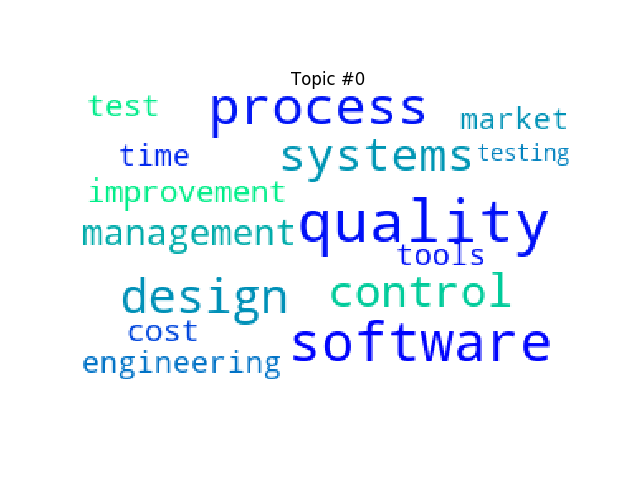
\includegraphics[width=0.35\textwidth]{figs/eu_topics/eu_FP4_wordclouds/EUFP4_topic0_7000.png}} &
\subfloat[Agriculture, Fisheries and Food]{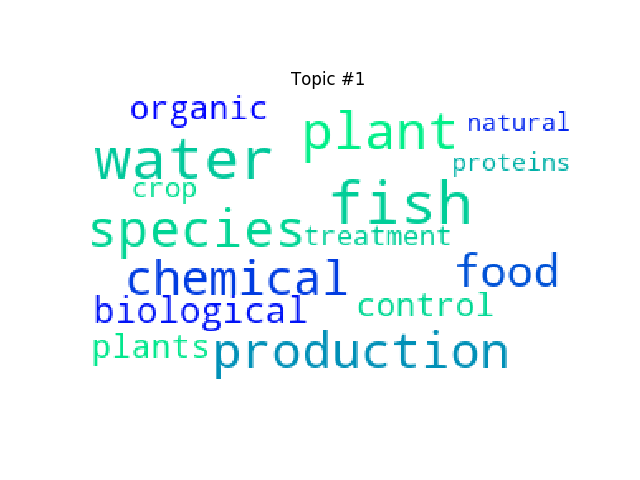
\includegraphics[width=0.35\textwidth]{figs/eu_topics/eu_FP4_wordclouds/EUFP4_topic1_7000.png}}&
\subfloat[Molecular biology, Genetics]{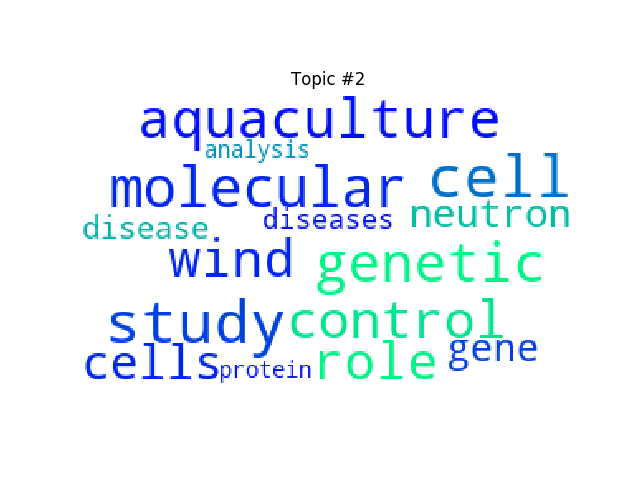
\includegraphics[width=0.35\textwidth]{figs/eu_topics/eu_FP4_wordclouds/EUFP4_topic2_7000.png}}\\
\subfloat[EU transport]{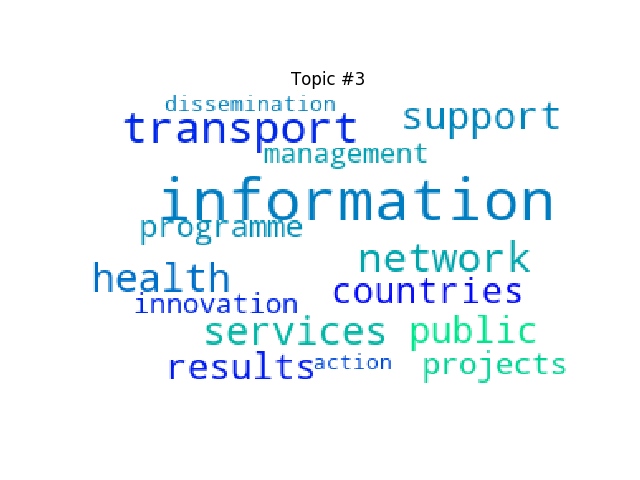
\includegraphics[width=0.35\textwidth]{figs/eu_topics/eu_FP4_wordclouds/EUFP4_topic3_7000.png}}&
\subfloat[Digital systems]{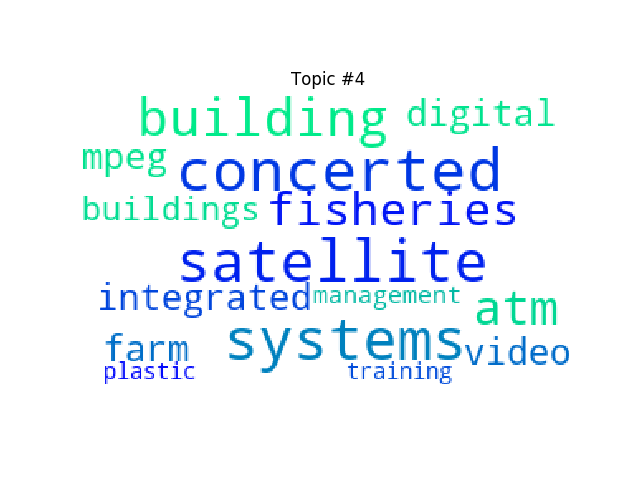
\includegraphics[width=0.35\textwidth]{figs/eu_topics/eu_FP4_wordclouds/EUFP4_topic4_7000.png}} &
\subfloat[Materials processing]{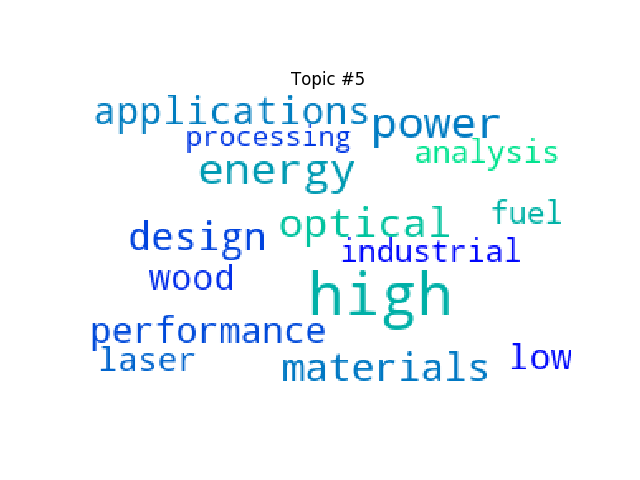
\includegraphics[width=0.35\textwidth]{figs/eu_topics/eu_FP4_wordclouds/EUFP4_topic5_7000.png}}\\
\subfloat[Genetics]{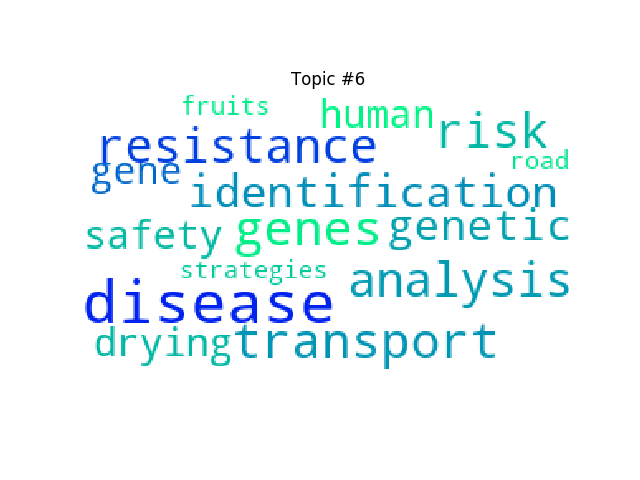
\includegraphics[width=0.35\textwidth]{figs/eu_topics/eu_FP4_wordclouds/EUFP4_topic6_7000.png}} &
\subfloat[Policy for environmental sustainability]{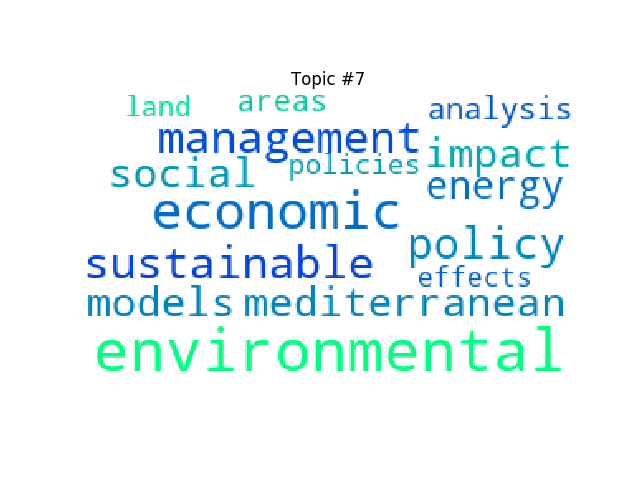
\includegraphics[width=0.35\textwidth]{figs/eu_topics/eu_FP4_wordclouds/EUFP4_topic7_7000.png}}&
\subfloat[Energy technologies]{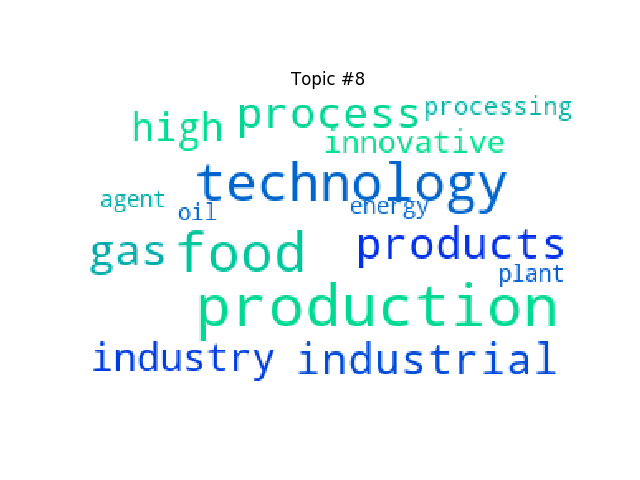
\includegraphics[width=0.35\textwidth]{figs/eu_topics/eu_FP4_wordclouds/EUFP4_topic8_7000.png}}\\
\subfloat[Applications in mobile networks]{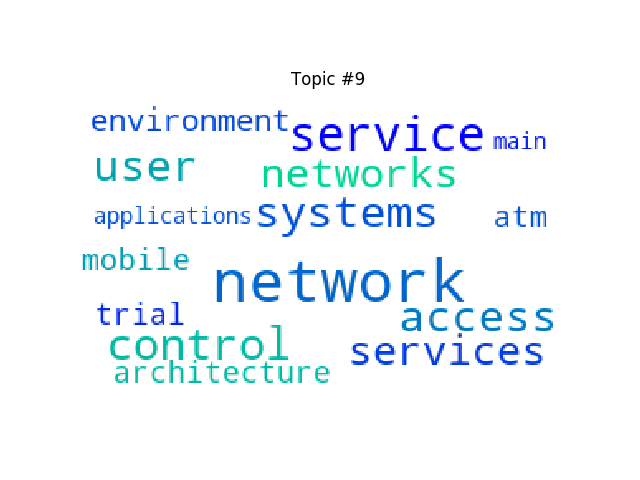
\includegraphics[width=0.35\textwidth]{figs/eu_topics/eu_FP4_wordclouds/EUFP4_topic9_7000.png}}&
\end{tabular}
\caption{Wordclouds of topics of the EU FP4 (1994-1998)}
\end{figure}
\end{center}

\begin{center}
\begin{figure}[h]
\begin{tabular}{rcl}
\subfloat[Management software]{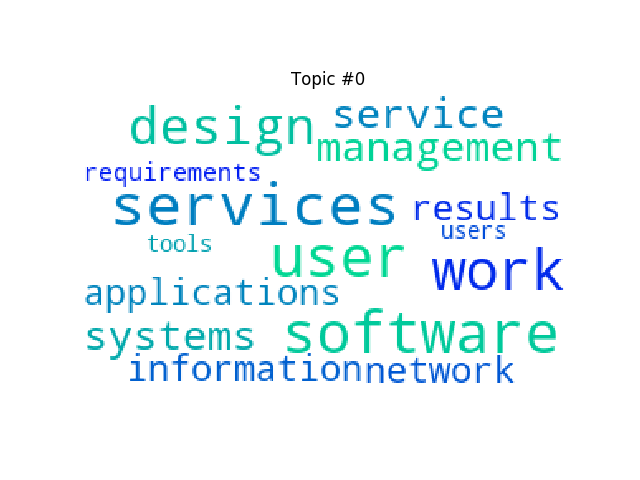
\includegraphics[width=0.35\textwidth]{figs/eu_topics/eu_FP5_wordclouds/EUFP5_topic0_7000.png}} &
\subfloat[Hydropower / Energy production]{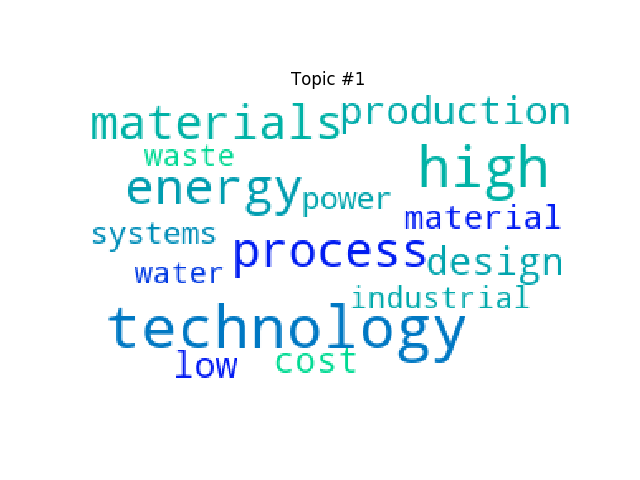
\includegraphics[width=0.35\textwidth]{figs/eu_topics/eu_FP5_wordclouds/EUFP5_topic1_7000.png}}&
\subfloat[Information technologies]{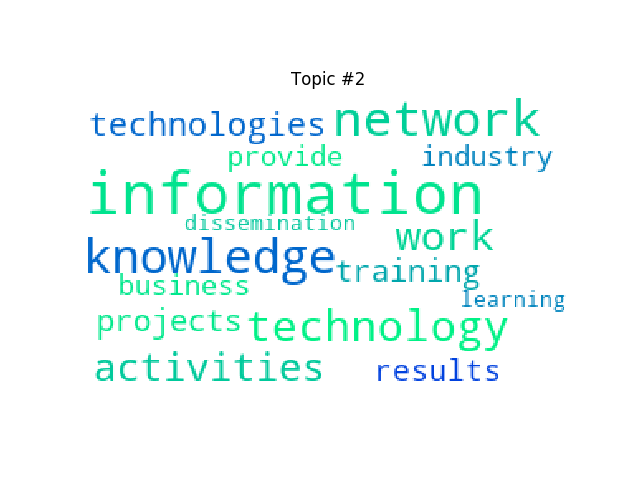
\includegraphics[width=0.35\textwidth]{figs/eu_topics/eu_FP5_wordclouds/EUFP5_topic2_7000.png}}\\
\subfloat[Quality control systems]{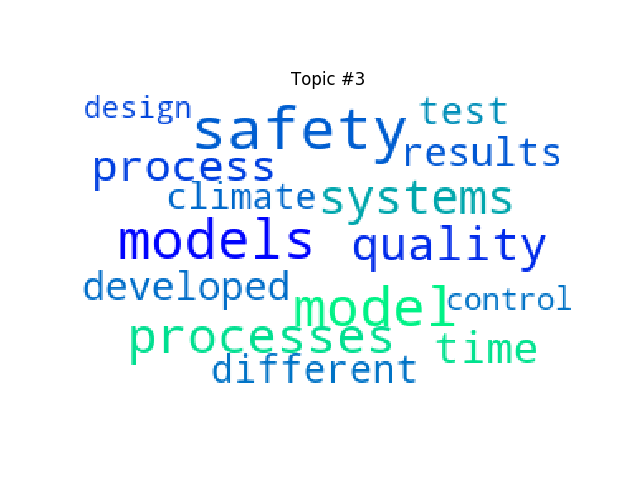
\includegraphics[width=0.35\textwidth]{figs/eu_topics/eu_FP5_wordclouds/EUFP5_topic3_7000.png}}&
\subfloat[Health care / Medical genetics]{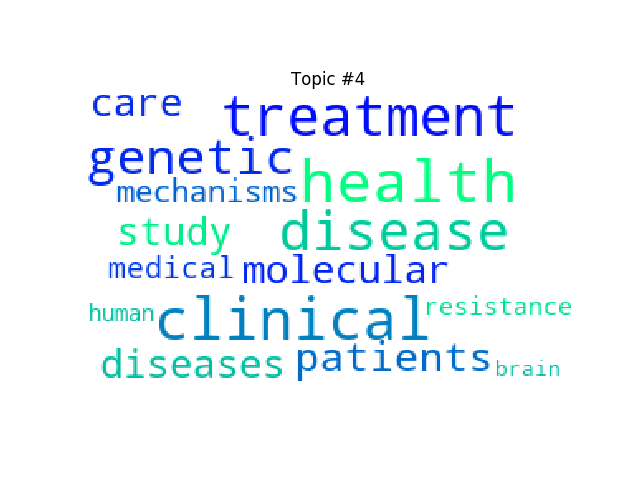
\includegraphics[width=0.35\textwidth]{figs/eu_topics/eu_FP5_wordclouds/EUFP5_topic4_7000.png}} &
\subfloat[Environmental sustainability and policies]{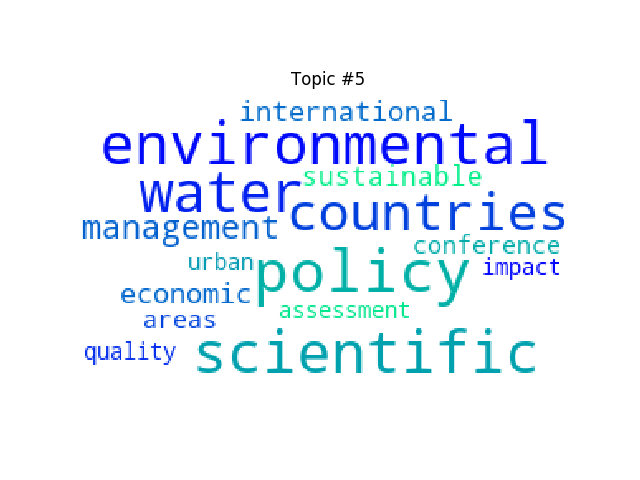
\includegraphics[width=0.35\textwidth]{figs/eu_topics/eu_FP5_wordclouds/EUFP5_topic5_7000.png}}\\
\subfloat[Molecular biology (genes)]{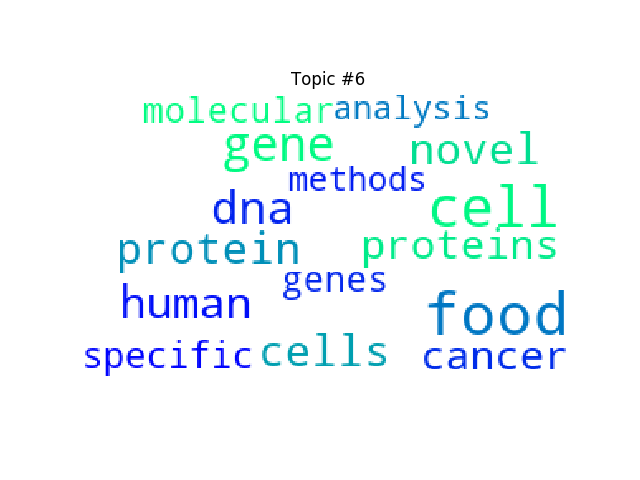
\includegraphics[width=0.35\textwidth]{figs/eu_topics/eu_FP5_wordclouds/EUFP5_topic6_7000.png}} &
\subfloat[Optical quantum computing]{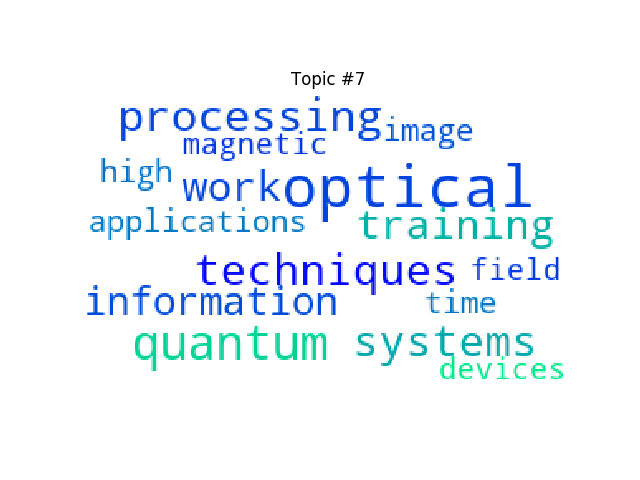
\includegraphics[width=0.35\textwidth]{figs/eu_topics/eu_FP5_wordclouds/EUFP5_topic7_7000.png}}&
\subfloat[Education in Nuclear physics]{\includegraphics[width=0.35\textwidth]{figs/eu_topics/eu_FP5_wordclouds/EUFP5_topic8_7000.png}}\\
\subfloat[Education, training]{\includegraphics[width=0.35\textwidth]{figs/eu_topics/eu_FP5_wordclouds/EUFP5_topic9_7000.png}}&
\end{tabular}
\caption{Wordclouds of topics of the EU FP5 (1998-2002)}
\end{figure}
\end{center}

\begin{center}
\begin{figure}[h]
\begin{tabular}{rcl}
\subfloat[International research]{\includegraphics[width=0.35\textwidth]{figs/eu_topics/eu_FP6_wordclouds/EUFP6_topic0_7000.png}} &
\subfloat[Biology]{\includegraphics[width=0.35\textwidth]{figs/eu_topics/eu_FP6_wordclouds/EUFP6_topic1_7000.png}}&
\subfloat[Embedded systems design]{\includegraphics[width=0.35\textwidth]{figs/eu_topics/eu_FP6_wordclouds/EUFP6_topic2_7000.png}}\\
\subfloat[Molecular biology, genes]{\includegraphics[width=0.35\textwidth]{figs/eu_topics/eu_FP6_wordclouds/EUFP6_topic3_7000.png}}&
\subfloat[Evolution / Formation]{\includegraphics[width=0.35\textwidth]{figs/eu_topics/eu_FP6_wordclouds/EUFP6_topic4_7000.png}} &
\subfloat[Sustainable production / Energy]{\includegraphics[width=0.35\textwidth]{figs/eu_topics/eu_FP6_wordclouds/EUFP6_topic5_7000.png}}\\
\subfloat[Economic \& Social policy]{\includegraphics[width=0.35\textwidth]{figs/eu_topics/eu_FP6_wordclouds/EUFP6_topic6_7000.png}} &
\subfloat[Environmental management services]{\includegraphics[width=0.35\textwidth]{figs/eu_topics/eu_FP6_wordclouds/EUFP6_topic7_7000.png}}&
\subfloat[Materials]{\includegraphics[width=0.35\textwidth]{figs/eu_topics/eu_FP6_wordclouds/EUFP6_topic8_7000.png}}\\
\subfloat[Cognitive neuroscience]{\includegraphics[width=0.35\textwidth]{figs/eu_topics/eu_FP6_wordclouds/EUFP6_topic9_7000.png}}&
\end{tabular}
\caption{Wordclouds of topics of the EU FP6 (2002-2006)}
\end{figure}
\end{center}

\begin{center}
\begin{figure}[h]
\begin{tabular}{rcl}
\subfloat[Cancer detection \& treatment]{\includegraphics[width=0.35\textwidth]{figs/eu_topics/eu_FP7_wordclouds/EUFP7_topic0_7000.png}} &
\subfloat[(High energy) physics]{\includegraphics[width=0.35\textwidth]{figs/eu_topics/eu_FP7_wordclouds/EUFP7_topic1_7000.png}}&
\subfloat[Energy production]{\includegraphics[width=0.35\textwidth]{figs/eu_topics/eu_FP7_wordclouds/EUFP7_topic2_7000.png}}\\
\subfloat[Social Sciences]{\includegraphics[width=0.35\textwidth]{figs/eu_topics/eu_FP7_wordclouds/EUFP7_topic3_7000.png}}&
\subfloat[Molecular Biology / Genetics]{\includegraphics[width=0.35\textwidth]{figs/eu_topics/eu_FP7_wordclouds/EUFP7_topic4_7000.png}} &
\subfloat[Information systems]{\includegraphics[width=0.35\textwidth]{figs/eu_topics/eu_FP7_wordclouds/EUFP7_topic5_7000.png}}\\
\subfloat[International research]{\includegraphics[width=0.35\textwidth]{figs/eu_topics/eu_FP7_wordclouds/EUFP7_topic6_7000.png}} &
\subfloat[Mathematics]{\includegraphics[width=0.35\textwidth]{figs/eu_topics/eu_FP7_wordclouds/EUFP7_topic7_7000.png}}&
\subfloat[Materials]{\includegraphics[width=0.35\textwidth]{figs/eu_topics/eu_FP7_wordclouds/EUFP7_topic8_7000.png}}\\
\subfloat[Molecular biology]{\includegraphics[width=0.35\textwidth]{figs/eu_topics/eu_FP7_wordclouds/EUFP7_topic9_7000.png}}&
\end{tabular}
\caption{Wordclouds of topics of the EU FP7 (2007-2013)}
\end{figure}
\end{center}

\begin{center}
\begin{figure}[h]
\begin{tabular}{rcl}
\subfloat[Molecular biology]{\includegraphics[width=0.35\textwidth]{figs/eu_topics/eu_H2020_wordclouds/EUH2020_topic0_20000.png}} &
\subfloat[Environmental sustainability \& food production]{\includegraphics[width=0.35\textwidth]{figs/eu_topics/eu_H2020_wordclouds/EUH2020_topic1_20000.png}}&
\subfloat[Information systems]{\includegraphics[width=0.35\textwidth]{figs/eu_topics/eu_H2020_wordclouds/EUH2020_topic2_20000.png}}\\
\subfloat[?]{\includegraphics[width=0.35\textwidth]{figs/eu_topics/eu_H2020_wordclouds/EUH2020_topic3_20000.png}}&
\subfloat[Materials]{\includegraphics[width=0.35\textwidth]{figs/eu_topics/eu_H2020_wordclouds/EUH2020_topic4_20000.png}} &
\subfloat[Environmental sustainability / Green energy]{\includegraphics[width=0.35\textwidth]{figs/eu_topics/eu_H2020_wordclouds/EUH2020_topic5_20000.png}}\\
\subfloat[Physics]{\includegraphics[width=0.35\textwidth]{figs/eu_topics/eu_H2020_wordclouds/EUH2020_topic6_20000.png}} &
\subfloat[Business \& Innovation]{\includegraphics[width=0.35\textwidth]{figs/eu_topics/eu_H2020_wordclouds/EUH2020_topic7_20000.png}}&
\subfloat[Cancer detection \& treatment]{\includegraphics[width=0.35\textwidth]{figs/eu_topics/eu_H2020_wordclouds/EUH2020_topic8_20000.png}}\\
\subfloat[Economic \& Social policy]{\includegraphics[width=0.35\textwidth]{figs/eu_topics/eu_H2020_wordclouds/EUH2020_topic9_20000.png}}&
\end{tabular}
\caption{Wordclouds of topics of the EU H2020 (2014-2020)}
\end{figure}
\end{center}

\begin{center}
\begin{figure}[h]
\begin{tabular}{rcl}
\subfloat[Software engineering]{\includegraphics[width=0.35\textwidth]{figs/usa_topics/usa_FP4_wordclouds/USAFP4_topic0_8000.png}} &
\subfloat[Climate change]{\includegraphics[width=0.35\textwidth]{figs/usa_topics/usa_FP4_wordclouds/USAFP4_topic1_8000.png}}&
\subfloat[International research \& Education]{\includegraphics[width=0.35\textwidth]{figs/usa_topics/usa_FP4_wordclouds/USAFP4_topic2_8000.png}}\\
\subfloat[Chemistry]{\includegraphics[width=0.35\textwidth]{figs/usa_topics/usa_FP4_wordclouds/USAFP4_topic3_8000.png}}&
\subfloat[Economic \& Social science]{\includegraphics[width=0.35\textwidth]{figs/usa_topics/usa_FP4_wordclouds/USAFP4_topic4_8000.png}} &
\subfloat[Mathematics]{\includegraphics[width=0.35\textwidth]{figs/usa_topics/usa_FP4_wordclouds/USAFP4_topic5_8000.png}}\\
\subfloat[Molecular biology / Genetics]{\includegraphics[width=0.35\textwidth]{figs/usa_topics/usa_FP4_wordclouds/USAFP4_topic6_8000.png}} &
\subfloat[Materials]{\includegraphics[width=0.35\textwidth]{figs/usa_topics/usa_FP4_wordclouds/USAFP4_topic7_8000.png}}&
\subfloat[Cognitive neuroscience]{\includegraphics[width=0.35\textwidth]{figs/usa_topics/usa_FP4_wordclouds/USAFP4_topic8_8000.png}}\\
\subfloat[High energy physics]{\includegraphics[width=0.35\textwidth]{figs/usa_topics/usa_FP4_wordclouds/USAFP4_topic9_8000.png}}&
\end{tabular}
\caption{Wordclouds of topics of the USA (1994-1997)}
\end{figure}
\end{center}

\begin{center}
\begin{figure}[h]
\begin{tabular}{rcl}
\subfloat[Applied Sciences]{\includegraphics[width=0.35\textwidth]{figs/usa_topics/usa_FP5_wordclouds/USAFP5_topic0_8000.png}} &
\subfloat[Environment \& Climate change]{\includegraphics[width=0.35\textwidth]{figs/usa_topics/usa_FP5_wordclouds/USAFP5_topic1_8000.png}}&
\subfloat[Materials \& Chemistry]{\includegraphics[width=0.35\textwidth]{figs/usa_topics/usa_FP5_wordclouds/USAFP5_topic2_8000.png}}\\
\subfloat[Biology]{\includegraphics[width=0.35\textwidth]{figs/usa_topics/usa_FP5_wordclouds/USAFP5_topic3_8000.png}}&
\subfloat[Information systems]{\includegraphics[width=0.35\textwidth]{figs/usa_topics/usa_FP5_wordclouds/USAFP5_topic4_8000.png}} &
\subfloat[STEM education]{\includegraphics[width=0.35\textwidth]{figs/usa_topics/usa_FP5_wordclouds/USAFP5_topic5_8000.png}}\\
\subfloat[Systems ?]{\includegraphics[width=0.35\textwidth]{figs/usa_topics/usa_FP5_wordclouds/USAFP5_topic6_8000.png}} &
\subfloat[Biology \& Evolution]{\includegraphics[width=0.35\textwidth]{figs/usa_topics/usa_FP5_wordclouds/USAFP5_topic7_8000.png}}&
\subfloat[Mathematics]{\includegraphics[width=0.35\textwidth]{figs/usa_topics/usa_FP5_wordclouds/USAFP5_topic8_8000.png}}\\
\subfloat[International conferences]{\includegraphics[width=0.35\textwidth]{figs/usa_topics/usa_FP5_wordclouds/USAFP5_topic9_8000.png}}&
\end{tabular}
\caption{Wordclouds of topics of the USA (1998-2001)}
\end{figure}
\end{center}

\begin{center}
\begin{figure}[h]
\begin{tabular}{rcl}
\subfloat[Information systems]{\includegraphics[width=0.35\textwidth]{figs/usa_topics/usa_FP6_wordclouds/USAFP6_topic0_8000.png}} &
\subfloat[Education (in engineering)]{\includegraphics[width=0.35\textwidth]{figs/usa_topics/usa_FP6_wordclouds/USAFP6_topic1_8000.png}}&
\subfloat[Materials \& Chemistry]{\includegraphics[width=0.35\textwidth]{figs/usa_topics/usa_FP6_wordclouds/USAFP6_topic2_8000.png}}\\
\subfloat[International conferences]{\includegraphics[width=0.35\textwidth]{figs/usa_topics/usa_FP6_wordclouds/USAFP6_topic3_8000.png}}&
\subfloat[Biology \& Evolution]{\includegraphics[width=0.35\textwidth]{figs/usa_topics/usa_FP6_wordclouds/USAFP6_topic4_8000.png}} &
\subfloat[Green transportation]{\includegraphics[width=0.35\textwidth]{figs/usa_topics/usa_FP6_wordclouds/USAFP6_topic5_8000.png}}\\
\subfloat[Economic \& Social policy]{\includegraphics[width=0.35\textwidth]{figs/usa_topics/usa_FP6_wordclouds/USAFP6_topic6_8000.png}} &
\subfloat[Climate change]{\includegraphics[width=0.35\textwidth]{figs/usa_topics/usa_FP6_wordclouds/USAFP6_topic7_8000.png}}&
\subfloat[Materials]{\includegraphics[width=0.35\textwidth]{figs/usa_topics/usa_FP6_wordclouds/USAFP6_topic8_8000.png}}\\
\subfloat[Physics]{\includegraphics[width=0.35\textwidth]{figs/usa_topics/usa_FP6_wordclouds/USAFP6_topic9_8000.png}}&
\end{tabular}
\caption{Wordclouds of topics of the USA (2002-2006)}
\end{figure}
\end{center}

\begin{center}
\begin{figure}[h]
\begin{tabular}{rcl}
\subfloat[STEM education]{\includegraphics[width=0.35\textwidth]{figs/usa_topics/usa_FP7_wordclouds/USAFP7_topic0_9000.png}} &
\subfloat[Computer \& Networking systems]{\includegraphics[width=0.35\textwidth]{figs/usa_topics/usa_FP7_wordclouds/USAFP7_topic1_9000.png}}&
\subfloat[Chemistry \& Materials science]{\includegraphics[width=0.35\textwidth]{figs/usa_topics/usa_FP7_wordclouds/USAFP7_topic2_9000.png}}\\
\subfloat[Climate change \ Environmental science]{\includegraphics[width=0.35\textwidth]{figs/usa_topics/usa_FP7_wordclouds/USAFP7_topic3_9000.png}}&
\subfloat[High energy physics]{\includegraphics[width=0.35\textwidth]{figs/usa_topics/usa_FP7_wordclouds/USAFP7_topic4_9000.png}} &
\subfloat[Atmospheric \& Ocean sciences]{\includegraphics[width=0.35\textwidth]{figs/usa_topics/usa_FP7_wordclouds/USAFP7_topic5_9000.png}}\\
\subfloat[Information systems]{\includegraphics[width=0.35\textwidth]{figs/usa_topics/usa_FP7_wordclouds/USAFP7_topic6_9000.png}} &
\subfloat[Mathematics]{\includegraphics[width=0.35\textwidth]{figs/usa_topics/usa_FP7_wordclouds/USAFP7_topic7_9000.png}}&
\subfloat[(Molecular) biology]{\includegraphics[width=0.35\textwidth]{figs/usa_topics/usa_FP7_wordclouds/USAFP7_topic8_9000.png}}\\
\subfloat[Economic \& Social policy]{\includegraphics[width=0.35\textwidth]{figs/usa_topics/usa_FP7_wordclouds/USAFP7_topic9_9000.png}}&
\end{tabular}
\caption{Wordclouds of topics of the USA (2007-2013)}
\end{figure}
\end{center}

\begin{center}
\begin{figure}[h]
\begin{tabular}{rcl}
\subfloat[Biology]{\includegraphics[width=0.35\textwidth]{figs/usa_topics/usa_H2020_wordclouds/USAH2020_topic0_8000.png}} &
\subfloat[Climate Change / Geology]{\includegraphics[width=0.35\textwidth]{figs/usa_topics/usa_H2020_wordclouds/USAH2020_topic1_8000.png}}&
\subfloat[Sociology]{\includegraphics[width=0.35\textwidth]{figs/usa_topics/usa_H2020_wordclouds/USAH2020_topic2_8000.png}}\\
\subfloat[STEM education]{\includegraphics[width=0.35\textwidth]{figs/usa_topics/usa_H2020_wordclouds/USAH2020_topic3_8000.png}}&
\subfloat[Information systems]{\includegraphics[width=0.35\textwidth]{figs/usa_topics/usa_H2020_wordclouds/USAH2020_topic4_8000.png}} &
\subfloat[Chemical \& transport systems]{\includegraphics[width=0.35\textwidth]{figs/usa_topics/usa_H2020_wordclouds/USAH2020_topic5_8000.png}}\\
\subfloat[Materials \& Chemistry]{\includegraphics[width=0.35\textwidth]{figs/usa_topics/usa_H2020_wordclouds/USAH2020_topic6_8000.png}} &
\subfloat[Materials \& Mechanical engineering]{\includegraphics[width=0.35\textwidth]{figs/usa_topics/usa_H2020_wordclouds/USAH2020_topic7_8000.png}}&
\subfloat[Mathematics]{\includegraphics[width=0.35\textwidth]{figs/usa_topics/usa_H2020_wordclouds/USAH2020_topic8_8000.png}}\\
\subfloat[International research]{\includegraphics[width=0.35\textwidth]{figs/usa_topics/usa_H2020_wordclouds/USAH2020_topic9_8000.png}}&
\end{tabular}
\caption{Wordclouds of topics of the USA (2014-2017)}
\end{figure}
\end{center}

\end{document}